\documentclass[12pt,a4paper]{article}
\usepackage[spanish]{babel}
\usepackage[utf8]{inputenc}
\usepackage[T1]{fontenc}
\usepackage[letterpaper,top=2cm,bottom=5cm,left=3cm,right=3cm]{geometry}
\usepackage{graphicx,booktabs,array,xcolor,amsmath,hyperref}
\usepackage{titlesec,fancyhdr,parskip,enumitem,tcolorbox}
\usepackage{caption,float,subcaption,microtype}
\tcbuselibrary{skins,breakable}
\newtcolorbox{cajainfo}[1]{colback=black!5,colframe=black,
  fonttitle=\bfseries\small,title=#1,breakable,left=6pt,right=6pt}
\pagestyle{fancy}\fancyhf{}
\setlength{\headheight}{70pt}\renewcommand{\headrulewidth}{0.4pt}
\fancyhead[C]{%
  \begin{minipage}[c]{2.5cm}\centering
    
\includegraphics[width=2.2cm]{imagenes/uta.png}
  \end{minipage}\hfill
  \begin{minipage}[c]{8cm}\centering
    \small{\textbf{UNIVERSIDAD T\'ECNICA DE AMBATO}}\\[0.1cm]
    \scriptsize\textit{FACULTAD DE INGENIER\'IA EN SISTEMAS ELECTR\'ONICA E INDUSTRIAL}\\[0.1cm]
    \scriptsize\textbf{CARRERA DE SOFTWARE}\\[0.1cm]
    \scriptsize\textbf{CICLO ACAD\'EMICO: FEBRERO -- JULIO 2026}
  \end{minipage}\hfill
  \begin{minipage}[c]{2.5cm}\centering
    
\includegraphics[width=2.2cm]{imagenes/fisei.png}
  \end{minipage}}
\fancyfoot[C]{\thepage}
\titleformat{\section}{\large\bfseries}{\thesection}{1em}{}[\titlerule]
\titleformat{\subsection}{\normalsize\bfseries}{\thesubsection}{1em}{}
\begin{document}
\begin{center}{\large\textbf{INFORME DE GU\'IA PR\'ACTICA}}\end{center}
\section{Portada}
\begin{flushleft}\renewcommand{\arraystretch}{1.3}
\begin{tabular}{@{} l p{10cm} @{}}
  \textbf{Tema:} & Hip\'otesis Dic\'otomicas en Machine Learning \\
  \textbf{Unidad de Organizaci\'on Curricular:} & Profesional. \\
  \textbf{Nivel y Paralelo:} & 6to -- A \\
  \textbf{Alumnos:} & Toala Camacho Steeven Santiago. \\ & Alexis Eduardo Lopez Guerrero. \\
  \textbf{Asignatura:} & Inteligencia de Negocios \\
  \textbf{Docente:} & Ing. Rub\'en Nogales. \\
\end{tabular}\end{flushleft}
\section{Objetivos}
\subsection*{Objetivo General}
Analizar y visualizar las hip\'otesis dic\'otomicas linealmente separables
de tres conjuntos de puntos, identificando la funci\'on separadora y el vector
normal en cada caso.
\subsection*{Objetivos Espec\'ificos}
\begin{enumerate}[label=\arabic*.]
  \item Enumerar las $2^N$ dic\'otom\'ias posibles de cada conjunto.
  \item Verificar la separabilidad lineal de cada dic\'otom\'ia.
  \item Graficar la frontera de decisi\'on $h(\mathbf{x})$ y el vector normal $\mathbf{w}$.
  \item Analizar la funci\'on utilizada en cada hip\'otesis v\'alida.
\end{enumerate}
\section{Introducci\'on}
Una \textbf{hip\'otesis dic\'otomica} es una funci\'on $h:\mathcal{X}\to\{0,1\}$
que separa el espacio en dos clases. El clasificador lineal en 2D implementa:
\[ h(\mathbf{x}) = \begin{cases} 1 & \text{si } w_1 x_1 + w_2 x_2 + b \geq 0 \\ 0 & \text{si no} \end{cases} \]
La recta $w_1 x_1 + w_2 x_2 + b = 0$ es la \textbf{frontera de decisi\'on}.
El vector $\mathbf{w}=(w_1,w_2)$ es \textbf{perpendicular} a dicha recta y
apunta hacia la regi\'on de clase~1.

\begin{cajainfo}{Convenci\'on de etiquetas en las tablas}
\textbf{S} = Linealmente separable \quad \textbf{No} = No linealmente separable
\end{cajainfo}

\section{Grupo 1}
\subsection{Conjunto de puntos}
\begin{table}[H]\centering
  \caption{Coordenadas de Grupo 1}
  \begin{tabular}{ccc}\toprule
    \textbf{Punto} & \textbf{$x_1$} & \textbf{$x_2$}\\\midrule
    $X_{1}$ & 2 & 2 \\
    $X_{2}$ & 4 & 4 \\
    $X_{3}$ & 6 & 6 \\
    $X_{4}$ & 6 & 8 \\
  \bottomrule\end{tabular}
\end{table}

\subsection{Tabla de dic\'otom\'ias ($2^{4}=16$ posibles)}
\begin{table}[H]\centering
  \caption{Todas las dic\'otom\'ias posibles -- Grupo 1}
  \begin{tabular}{cccccc}\toprule
    \textbf{Dic.} & $X_{1}$ & $X_{2}$ & $X_{3}$ & $X_{4}$ & \textbf{Sep.}\\\midrule
    $D_{1}$ & 0 & 0 & 0 & 0 & \textbf{S} \\
    $D_{2}$ & 0 & 0 & 0 & 1 & \textbf{S} \\
    $D_{3}$ & 0 & 0 & 1 & 0 & \textbf{S} \\
    $D_{4}$ & 0 & 0 & 1 & 1 & \textbf{S} \\
    $D_{5}$ & 0 & 1 & 0 & 0 & No \\
    $D_{6}$ & 0 & 1 & 0 & 1 & No \\
    $D_{7}$ & 0 & 1 & 1 & 0 & \textbf{S} \\
    $D_{8}$ & 0 & 1 & 1 & 1 & \textbf{S} \\
    $D_{9}$ & 1 & 0 & 0 & 0 & \textbf{S} \\
    $D_{10}$ & 1 & 0 & 0 & 1 & \textbf{S} \\
    $D_{11}$ & 1 & 0 & 1 & 0 & No \\
    $D_{12}$ & 1 & 0 & 1 & 1 & No \\
    $D_{13}$ & 1 & 1 & 0 & 0 & \textbf{S} \\
    $D_{14}$ & 1 & 1 & 0 & 1 & \textbf{S} \\
    $D_{15}$ & 1 & 1 & 1 & 0 & \textbf{S} \\
    $D_{16}$ & 1 & 1 & 1 & 1 & \textbf{S} \\
  \bottomrule\end{tabular}
\end{table}

\subsection{Hip\'otesis v\'alidas}

\subsubsection{Hip\'otesis $H_{1}$: etiquetas [0, 0, 0, 0]}
\begin{table}[H]\centering
  \caption{Clasificaci\'on de $H_{1}$}
  \begin{tabular}{ccc}\toprule
    \textbf{Punto} & \textbf{Coordenadas} & \textbf{Clase}\\\midrule
    $X_{1}$ & (2, 2) & 0 \\
    $X_{2}$ & (4, 4) & 0 \\
    $X_{3}$ & (6, 6) & 0 \\
    $X_{4}$ & (6, 8) & 0 \\
  \bottomrule\end{tabular}
\end{table}
\begin{figure}[H]\centering
  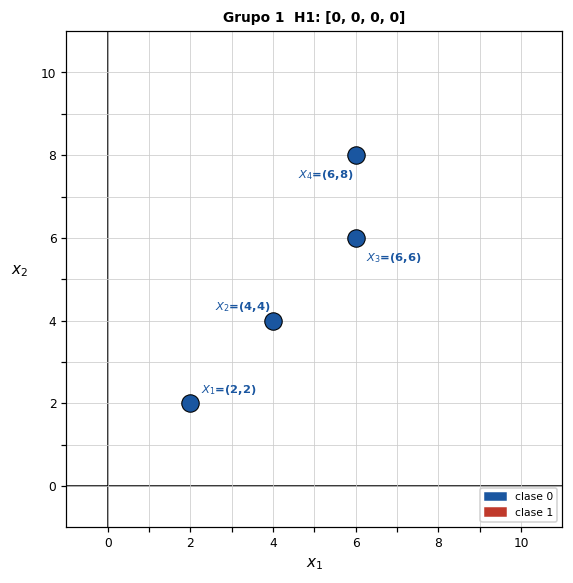
\includegraphics[width=0.65\textwidth]{imagenes_hipotesis/Grupo_1_H01.png}
  \caption{$H_{1}$ -- Grupo 1}
\end{figure}
\textbf{An\'alisis:}
\begin{itemize}
  \item Esta hip\'otesis es \textbf{trivial}: todos los puntos pertenecen a la misma clase.
  \item No existe frontera de decisi\'on expl\'icita.
\end{itemize}

\subsubsection{Hip\'otesis $H_{2}$: etiquetas [0, 0, 0, 1]}
\begin{table}[H]\centering
  \caption{Clasificaci\'on de $H_{2}$}
  \begin{tabular}{ccc}\toprule
    \textbf{Punto} & \textbf{Coordenadas} & \textbf{Clase}\\\midrule
    $X_{1}$ & (2, 2) & 0 \\
    $X_{2}$ & (4, 4) & 0 \\
    $X_{3}$ & (6, 6) & 0 \\
    $X_{4}$ & (6, 8) & 1 \\
  \bottomrule\end{tabular}
\end{table}
\begin{figure}[H]\centering
  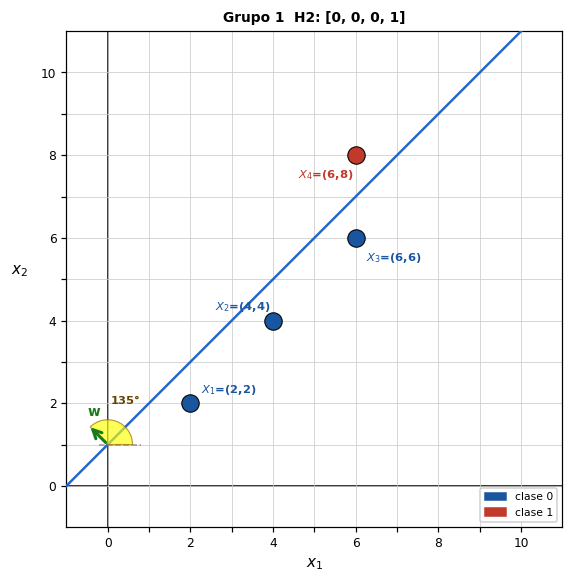
\includegraphics[width=0.65\textwidth]{imagenes_hipotesis/Grupo_1_H02.png}
  \caption{$H_{2}$ -- Grupo 1}
\end{figure}
\textbf{An\'alisis:}
\begin{itemize}
  \item \textbf{Funci\'on separadora:} $-1.00 x_1 + 1.00 x_2 - 1.00 = 0$
  \item \textbf{Vector normal:} $\mathbf{w} = (-1.000, 1.000)$, perpendicular a la recta.
  \item \textbf{\'Angulo:} $\theta = 135.0 grados$.
  \item \textbf{Direcci\'on de $\mathbf{w}$:} El vector $\mathbf{w}$ apunta hacia el \textbf{cuadrante superior-izquierdo} ($x_1$ negativo, $x_2$ positivo). La clase~1 se encuentra a la izquierda y arriba de la frontera.
  \item \textbf{Clase 0} (lado negativo): $X_{1}$, $X_{2}$, $X_{3}$
  \item \textbf{Clase 1} (lado positivo, direcci\'on de $\mathbf{w}$): $X_{4}$
\end{itemize}

\subsubsection{Hip\'otesis $H_{3}$: etiquetas [0, 0, 1, 0]}
\begin{table}[H]\centering
  \caption{Clasificaci\'on de $H_{3}$}
  \begin{tabular}{ccc}\toprule
    \textbf{Punto} & \textbf{Coordenadas} & \textbf{Clase}\\\midrule
    $X_{1}$ & (2, 2) & 0 \\
    $X_{2}$ & (4, 4) & 0 \\
    $X_{3}$ & (6, 6) & 1 \\
    $X_{4}$ & (6, 8) & 0 \\
  \bottomrule\end{tabular}
\end{table}
\begin{figure}[H]\centering
  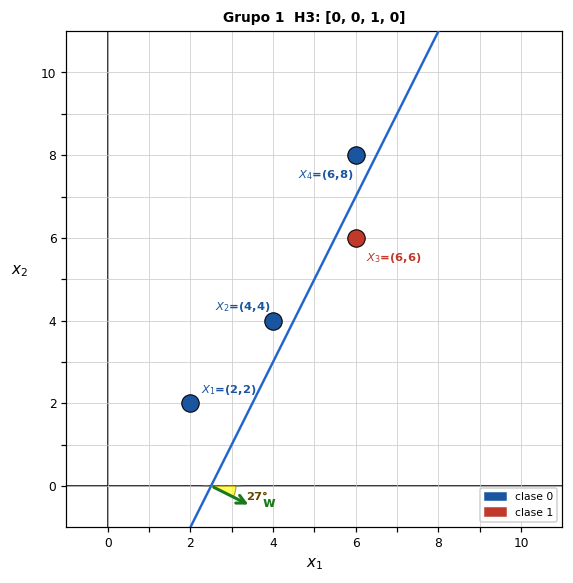
\includegraphics[width=0.65\textwidth]{imagenes_hipotesis/Grupo_1_H03.png}
  \caption{$H_{3}$ -- Grupo 1}
\end{figure}
\textbf{An\'alisis:}
\begin{itemize}
  \item \textbf{Funci\'on separadora:} $2.00 x_1 - 1.00 x_2 - 5.00 = 0$
  \item \textbf{Vector normal:} $\mathbf{w} = (2.000, -1.000)$, perpendicular a la recta.
  \item \textbf{\'Angulo:} $\theta = 333.4 grados$.
  \item \textbf{Direcci\'on de $\mathbf{w}$:} El vector $\mathbf{w}$ apunta hacia el \textbf{cuadrante inferior-derecho} ($x_1$ positivo, $x_2$ negativo). La clase~1 se encuentra en la regi'on inferior-derecha.
  \item \textbf{Clase 0} (lado negativo): $X_{1}$, $X_{2}$, $X_{4}$
  \item \textbf{Clase 1} (lado positivo, direcci\'on de $\mathbf{w}$): $X_{3}$
\end{itemize}

\subsubsection{Hip\'otesis $H_{4}$: etiquetas [0, 0, 1, 1]}
\begin{table}[H]\centering
  \caption{Clasificaci\'on de $H_{4}$}
  \begin{tabular}{ccc}\toprule
    \textbf{Punto} & \textbf{Coordenadas} & \textbf{Clase}\\\midrule
    $X_{1}$ & (2, 2) & 0 \\
    $X_{2}$ & (4, 4) & 0 \\
    $X_{3}$ & (6, 6) & 1 \\
    $X_{4}$ & (6, 8) & 1 \\
  \bottomrule\end{tabular}
\end{table}
\begin{figure}[H]\centering
  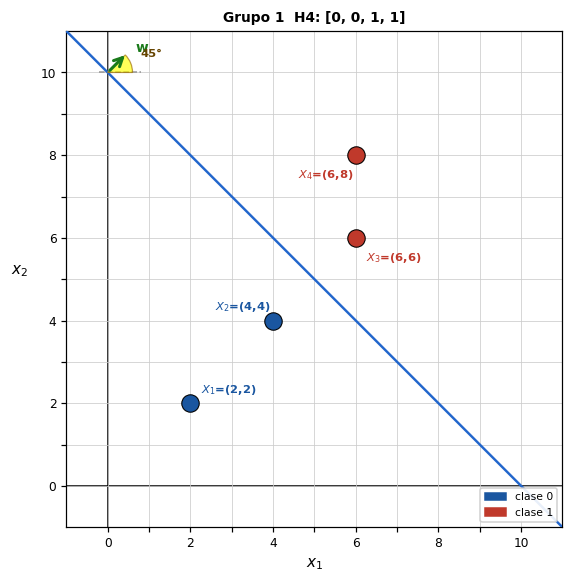
\includegraphics[width=0.65\textwidth]{imagenes_hipotesis/Grupo_1_H04.png}
  \caption{$H_{4}$ -- Grupo 1}
\end{figure}
\textbf{An\'alisis:}
\begin{itemize}
  \item \textbf{Funci\'on separadora:} $0.50 x_1 + 0.50 x_2 - 5.00 = 0$
  \item \textbf{Vector normal:} $\mathbf{w} = (0.500, 0.500)$, perpendicular a la recta.
  \item \textbf{\'Angulo:} $\theta = 45.0 grados$.
  \item \textbf{Direcci\'on de $\mathbf{w}$:} El vector $\mathbf{w}$ apunta hacia el \textbf{cuadrante superior-derecho} ($x_1$ positivo, $x_2$ positivo). La clase~1 se encuentra en esa direcci'on respecto a la frontera.
  \item \textbf{Clase 0} (lado negativo): $X_{1}$, $X_{2}$
  \item \textbf{Clase 1} (lado positivo, direcci\'on de $\mathbf{w}$): $X_{3}$, $X_{4}$
\end{itemize}

\subsubsection{Hip\'otesis $H_{5}$: etiquetas [0, 1, 1, 0]}
\begin{table}[H]\centering
  \caption{Clasificaci\'on de $H_{5}$}
  \begin{tabular}{ccc}\toprule
    \textbf{Punto} & \textbf{Coordenadas} & \textbf{Clase}\\\midrule
    $X_{1}$ & (2, 2) & 0 \\
    $X_{2}$ & (4, 4) & 1 \\
    $X_{3}$ & (6, 6) & 1 \\
    $X_{4}$ & (6, 8) & 0 \\
  \bottomrule\end{tabular}
\end{table}
\begin{figure}[H]\centering
  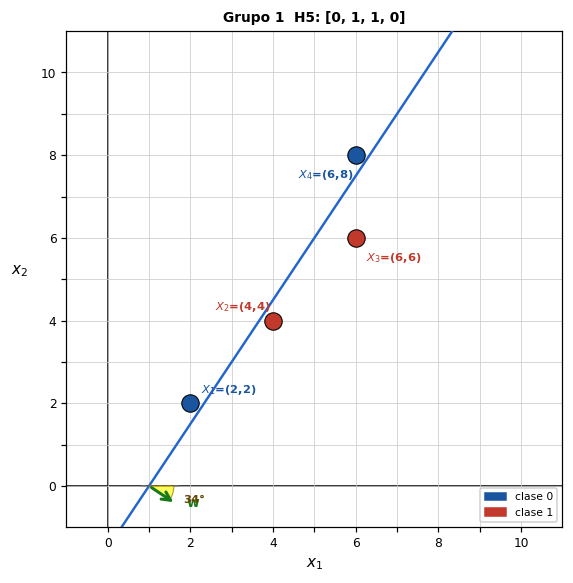
\includegraphics[width=0.65\textwidth]{imagenes_hipotesis/Grupo_1_H05.png}
  \caption{$H_{5}$ -- Grupo 1}
\end{figure}
\textbf{An\'alisis:}
\begin{itemize}
  \item \textbf{Funci\'on separadora:} $3.00 x_1 - 2.00 x_2 - 3.00 = 0$
  \item \textbf{Vector normal:} $\mathbf{w} = (3.000, -2.000)$, perpendicular a la recta.
  \item \textbf{\'Angulo:} $\theta = 326.3 grados$.
  \item \textbf{Direcci\'on de $\mathbf{w}$:} El vector $\mathbf{w}$ apunta hacia el \textbf{cuadrante inferior-derecho} ($x_1$ positivo, $x_2$ negativo). La clase~1 se encuentra en la regi'on inferior-derecha.
  \item \textbf{Clase 0} (lado negativo): $X_{1}$, $X_{4}$
  \item \textbf{Clase 1} (lado positivo, direcci\'on de $\mathbf{w}$): $X_{2}$, $X_{3}$
\end{itemize}

\subsubsection{Hip\'otesis $H_{6}$: etiquetas [0, 1, 1, 1]}
\begin{table}[H]\centering
  \caption{Clasificaci\'on de $H_{6}$}
  \begin{tabular}{ccc}\toprule
    \textbf{Punto} & \textbf{Coordenadas} & \textbf{Clase}\\\midrule
    $X_{1}$ & (2, 2) & 0 \\
    $X_{2}$ & (4, 4) & 1 \\
    $X_{3}$ & (6, 6) & 1 \\
    $X_{4}$ & (6, 8) & 1 \\
  \bottomrule\end{tabular}
\end{table}
\begin{figure}[H]\centering
  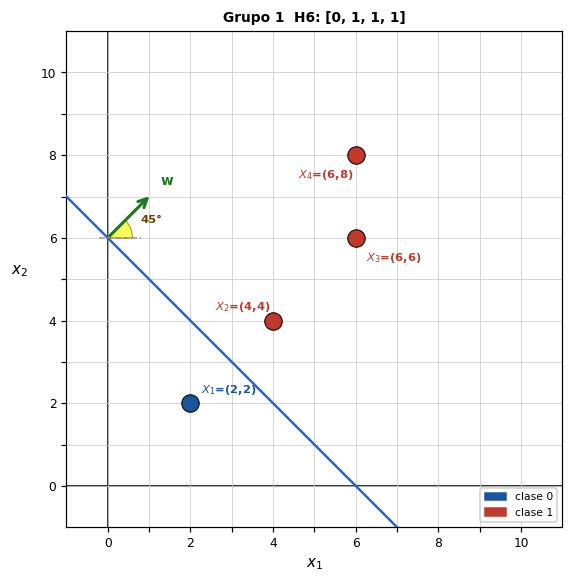
\includegraphics[width=0.65\textwidth]{imagenes_hipotesis/Grupo_1_H06.png}
  \caption{$H_{6}$ -- Grupo 1}
\end{figure}
\textbf{An\'alisis:}
\begin{itemize}
  \item \textbf{Funci\'on separadora:} $0.50 x_1 + 0.50 x_2 - 3.00 = 0$
  \item \textbf{Vector normal:} $\mathbf{w} = (0.500, 0.500)$, perpendicular a la recta.
  \item \textbf{\'Angulo:} $\theta = 45.0 grados$.
  \item \textbf{Direcci\'on de $\mathbf{w}$:} El vector $\mathbf{w}$ apunta hacia el \textbf{cuadrante superior-derecho} ($x_1$ positivo, $x_2$ positivo). La clase~1 se encuentra en esa direcci'on respecto a la frontera.
  \item \textbf{Clase 0} (lado negativo): $X_{1}$
  \item \textbf{Clase 1} (lado positivo, direcci\'on de $\mathbf{w}$): $X_{2}$, $X_{3}$, $X_{4}$
\end{itemize}

\subsubsection{Hip\'otesis $H_{7}$: etiquetas [1, 0, 0, 0]}
\begin{table}[H]\centering
  \caption{Clasificaci\'on de $H_{7}$}
  \begin{tabular}{ccc}\toprule
    \textbf{Punto} & \textbf{Coordenadas} & \textbf{Clase}\\\midrule
    $X_{1}$ & (2, 2) & 1 \\
    $X_{2}$ & (4, 4) & 0 \\
    $X_{3}$ & (6, 6) & 0 \\
    $X_{4}$ & (6, 8) & 0 \\
  \bottomrule\end{tabular}
\end{table}
\begin{figure}[H]\centering
  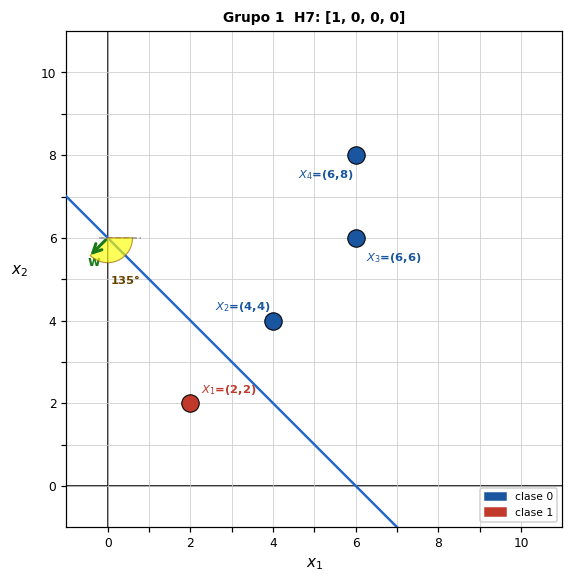
\includegraphics[width=0.65\textwidth]{imagenes_hipotesis/Grupo_1_H07.png}
  \caption{$H_{7}$ -- Grupo 1}
\end{figure}
\textbf{An\'alisis:}
\begin{itemize}
  \item \textbf{Funci\'on separadora:} $-0.50 x_1 - 0.50 x_2 + 3.00 = 0$
  \item \textbf{Vector normal:} $\mathbf{w} = (-0.500, -0.500)$, perpendicular a la recta.
  \item \textbf{\'Angulo:} $\theta = 225.0 grados$.
  \item \textbf{Direcci\'on de $\mathbf{w}$:} El vector $\mathbf{w}$ apunta hacia el \textbf{cuadrante inferior-izquierdo} ($x_1$ negativo, $x_2$ negativo). La clase~1 se encuentra en la regi'on inferior-izquierda.
  \item \textbf{Clase 0} (lado negativo): $X_{2}$, $X_{3}$, $X_{4}$
  \item \textbf{Clase 1} (lado positivo, direcci\'on de $\mathbf{w}$): $X_{1}$
\end{itemize}

\subsubsection{Hip\'otesis $H_{8}$: etiquetas [1, 0, 0, 1]}
\begin{table}[H]\centering
  \caption{Clasificaci\'on de $H_{8}$}
  \begin{tabular}{ccc}\toprule
    \textbf{Punto} & \textbf{Coordenadas} & \textbf{Clase}\\\midrule
    $X_{1}$ & (2, 2) & 1 \\
    $X_{2}$ & (4, 4) & 0 \\
    $X_{3}$ & (6, 6) & 0 \\
    $X_{4}$ & (6, 8) & 1 \\
  \bottomrule\end{tabular}
\end{table}
\begin{figure}[H]\centering
  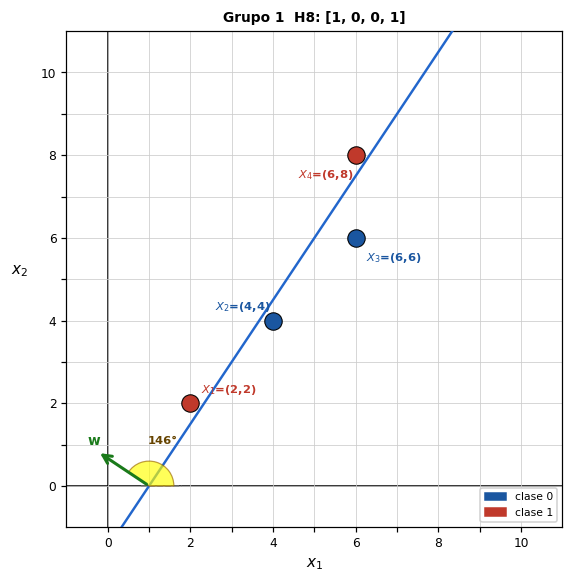
\includegraphics[width=0.65\textwidth]{imagenes_hipotesis/Grupo_1_H08.png}
  \caption{$H_{8}$ -- Grupo 1}
\end{figure}
\textbf{An\'alisis:}
\begin{itemize}
  \item \textbf{Funci\'on separadora:} $-3.00 x_1 + 2.00 x_2 + 3.00 = 0$
  \item \textbf{Vector normal:} $\mathbf{w} = (-3.000, 2.000)$, perpendicular a la recta.
  \item \textbf{\'Angulo:} $\theta = 146.3 grados$.
  \item \textbf{Direcci\'on de $\mathbf{w}$:} El vector $\mathbf{w}$ apunta hacia el \textbf{cuadrante superior-izquierdo} ($x_1$ negativo, $x_2$ positivo). La clase~1 se encuentra a la izquierda y arriba de la frontera.
  \item \textbf{Clase 0} (lado negativo): $X_{2}$, $X_{3}$
  \item \textbf{Clase 1} (lado positivo, direcci\'on de $\mathbf{w}$): $X_{1}$, $X_{4}$
\end{itemize}

\subsubsection{Hip\'otesis $H_{9}$: etiquetas [1, 1, 0, 0]}
\begin{table}[H]\centering
  \caption{Clasificaci\'on de $H_{9}$}
  \begin{tabular}{ccc}\toprule
    \textbf{Punto} & \textbf{Coordenadas} & \textbf{Clase}\\\midrule
    $X_{1}$ & (2, 2) & 1 \\
    $X_{2}$ & (4, 4) & 1 \\
    $X_{3}$ & (6, 6) & 0 \\
    $X_{4}$ & (6, 8) & 0 \\
  \bottomrule\end{tabular}
\end{table}
\begin{figure}[H]\centering
  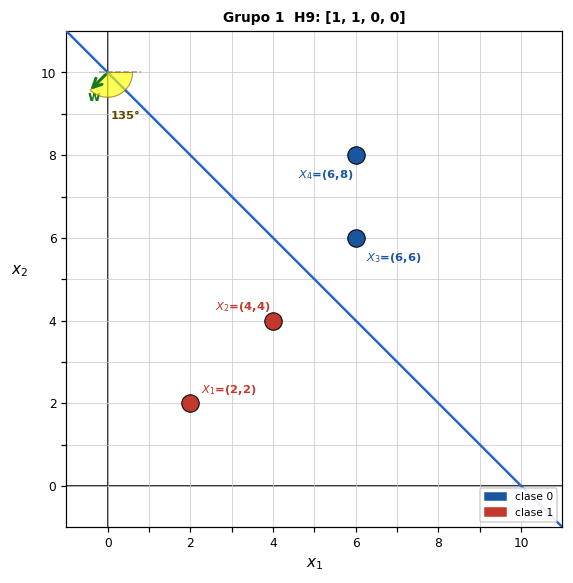
\includegraphics[width=0.65\textwidth]{imagenes_hipotesis/Grupo_1_H09.png}
  \caption{$H_{9}$ -- Grupo 1}
\end{figure}
\textbf{An\'alisis:}
\begin{itemize}
  \item \textbf{Funci\'on separadora:} $-0.50 x_1 - 0.50 x_2 + 5.00 = 0$
  \item \textbf{Vector normal:} $\mathbf{w} = (-0.500, -0.500)$, perpendicular a la recta.
  \item \textbf{\'Angulo:} $\theta = 225.0 grados$.
  \item \textbf{Direcci\'on de $\mathbf{w}$:} El vector $\mathbf{w}$ apunta hacia el \textbf{cuadrante inferior-izquierdo} ($x_1$ negativo, $x_2$ negativo). La clase~1 se encuentra en la regi'on inferior-izquierda.
  \item \textbf{Clase 0} (lado negativo): $X_{3}$, $X_{4}$
  \item \textbf{Clase 1} (lado positivo, direcci\'on de $\mathbf{w}$): $X_{1}$, $X_{2}$
\end{itemize}

\subsubsection{Hip\'otesis $H_{10}$: etiquetas [1, 1, 0, 1]}
\begin{table}[H]\centering
  \caption{Clasificaci\'on de $H_{10}$}
  \begin{tabular}{ccc}\toprule
    \textbf{Punto} & \textbf{Coordenadas} & \textbf{Clase}\\\midrule
    $X_{1}$ & (2, 2) & 1 \\
    $X_{2}$ & (4, 4) & 1 \\
    $X_{3}$ & (6, 6) & 0 \\
    $X_{4}$ & (6, 8) & 1 \\
  \bottomrule\end{tabular}
\end{table}
\begin{figure}[H]\centering
  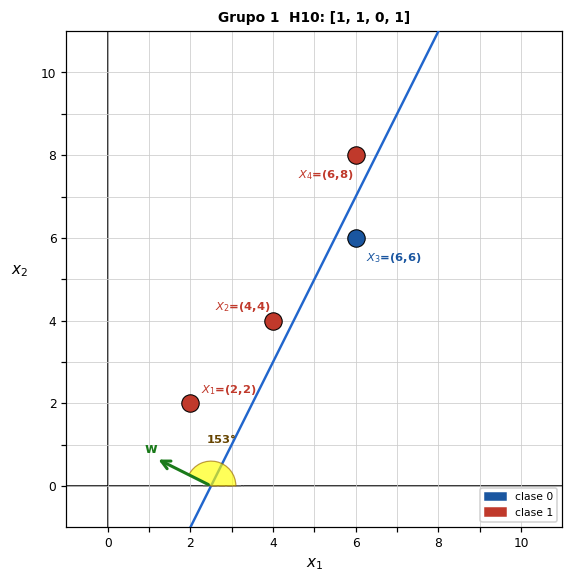
\includegraphics[width=0.65\textwidth]{imagenes_hipotesis/Grupo_1_H10.png}
  \caption{$H_{10}$ -- Grupo 1}
\end{figure}
\textbf{An\'alisis:}
\begin{itemize}
  \item \textbf{Funci\'on separadora:} $-2.00 x_1 + 1.00 x_2 + 5.00 = 0$
  \item \textbf{Vector normal:} $\mathbf{w} = (-2.000, 1.000)$, perpendicular a la recta.
  \item \textbf{\'Angulo:} $\theta = 153.4 grados$.
  \item \textbf{Direcci\'on de $\mathbf{w}$:} El vector $\mathbf{w}$ apunta hacia el \textbf{cuadrante superior-izquierdo} ($x_1$ negativo, $x_2$ positivo). La clase~1 se encuentra a la izquierda y arriba de la frontera.
  \item \textbf{Clase 0} (lado negativo): $X_{3}$
  \item \textbf{Clase 1} (lado positivo, direcci\'on de $\mathbf{w}$): $X_{1}$, $X_{2}$, $X_{4}$
\end{itemize}

\subsubsection{Hip\'otesis $H_{11}$: etiquetas [1, 1, 1, 0]}
\begin{table}[H]\centering
  \caption{Clasificaci\'on de $H_{11}$}
  \begin{tabular}{ccc}\toprule
    \textbf{Punto} & \textbf{Coordenadas} & \textbf{Clase}\\\midrule
    $X_{1}$ & (2, 2) & 1 \\
    $X_{2}$ & (4, 4) & 1 \\
    $X_{3}$ & (6, 6) & 1 \\
    $X_{4}$ & (6, 8) & 0 \\
  \bottomrule\end{tabular}
\end{table}
\begin{figure}[H]\centering
  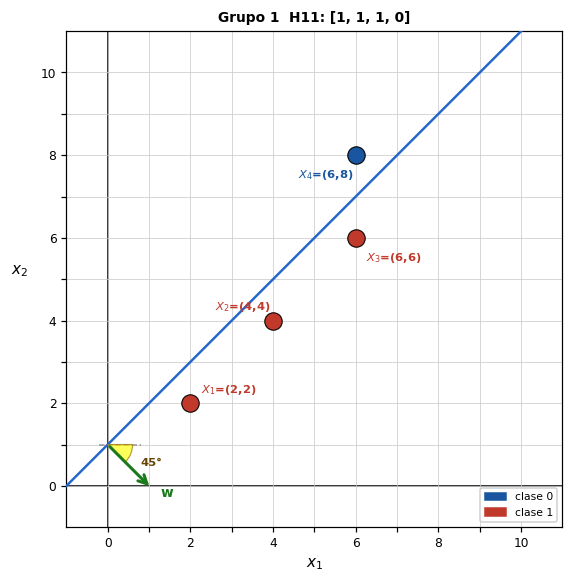
\includegraphics[width=0.65\textwidth]{imagenes_hipotesis/Grupo_1_H11.png}
  \caption{$H_{11}$ -- Grupo 1}
\end{figure}
\textbf{An\'alisis:}
\begin{itemize}
  \item \textbf{Funci\'on separadora:} $1.00 x_1 - 1.00 x_2 + 1.00 = 0$
  \item \textbf{Vector normal:} $\mathbf{w} = (1.000, -1.000)$, perpendicular a la recta.
  \item \textbf{\'Angulo:} $\theta = 315.0 grados$.
  \item \textbf{Direcci\'on de $\mathbf{w}$:} El vector $\mathbf{w}$ apunta hacia el \textbf{cuadrante inferior-derecho} ($x_1$ positivo, $x_2$ negativo). La clase~1 se encuentra en la regi'on inferior-derecha.
  \item \textbf{Clase 0} (lado negativo): $X_{4}$
  \item \textbf{Clase 1} (lado positivo, direcci\'on de $\mathbf{w}$): $X_{1}$, $X_{2}$, $X_{3}$
\end{itemize}

\subsubsection{Hip\'otesis $H_{12}$: etiquetas [1, 1, 1, 1]}
\begin{table}[H]\centering
  \caption{Clasificaci\'on de $H_{12}$}
  \begin{tabular}{ccc}\toprule
    \textbf{Punto} & \textbf{Coordenadas} & \textbf{Clase}\\\midrule
    $X_{1}$ & (2, 2) & 1 \\
    $X_{2}$ & (4, 4) & 1 \\
    $X_{3}$ & (6, 6) & 1 \\
    $X_{4}$ & (6, 8) & 1 \\
  \bottomrule\end{tabular}
\end{table}
\begin{figure}[H]\centering
  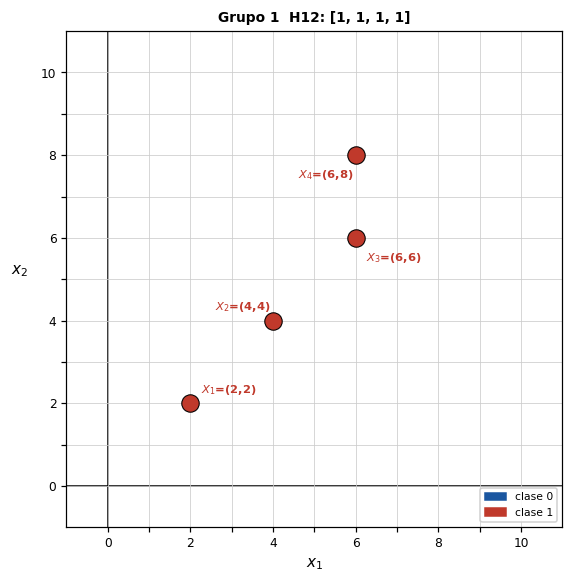
\includegraphics[width=0.65\textwidth]{imagenes_hipotesis/Grupo_1_H12.png}
  \caption{$H_{12}$ -- Grupo 1}
\end{figure}
\textbf{An\'alisis:}
\begin{itemize}
  \item Esta hip\'otesis es \textbf{trivial}: todos los puntos pertenecen a la misma clase.
  \item No existe frontera de decisi\'on expl\'icita.
\end{itemize}

\subsection{Hip\'otesis NO Linealmente Separables}
Las siguientes dic\'otom\'ias \textbf{no pueden ser realizadas}
por ning\'un clasificador lineal sobre este conjunto de puntos.
\begin{figure}[H]\centering
  \begin{subfigure}[b]{0.47\textwidth}
    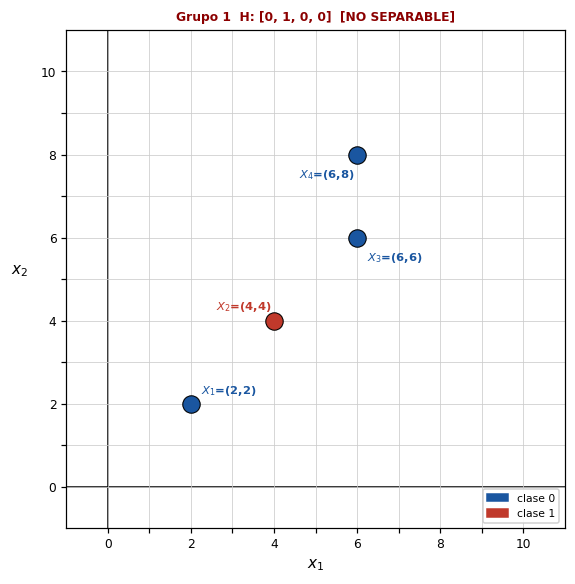
\includegraphics[width=\textwidth]{imagenes_hipotesis/Grupo_1_NS01.png}
    \caption{No separable: [0, 1, 0, 0]}
  \end{subfigure}\hfill
  \begin{subfigure}[b]{0.47\textwidth}
    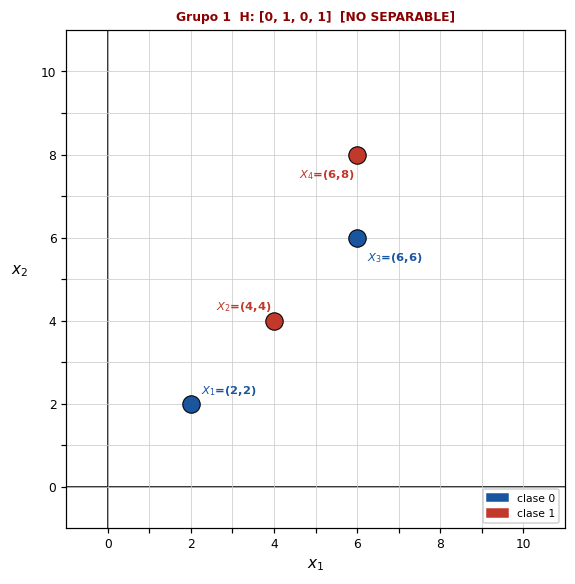
\includegraphics[width=\textwidth]{imagenes_hipotesis/Grupo_1_NS02.png}
    \caption{No separable: [0, 1, 0, 1]}
  \end{subfigure}\hfill
\end{figure}

\begin{figure}[H]\centering
  \begin{subfigure}[b]{0.47\textwidth}
    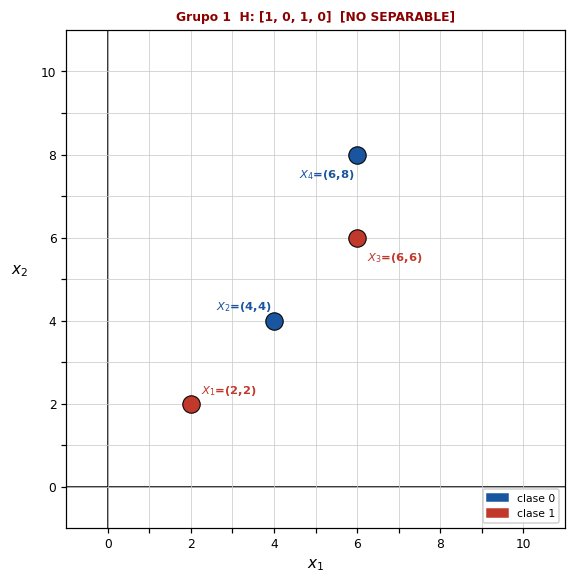
\includegraphics[width=\textwidth]{imagenes_hipotesis/Grupo_1_NS03.png}
    \caption{No separable: [1, 0, 1, 0]}
  \end{subfigure}\hfill
  \begin{subfigure}[b]{0.47\textwidth}
    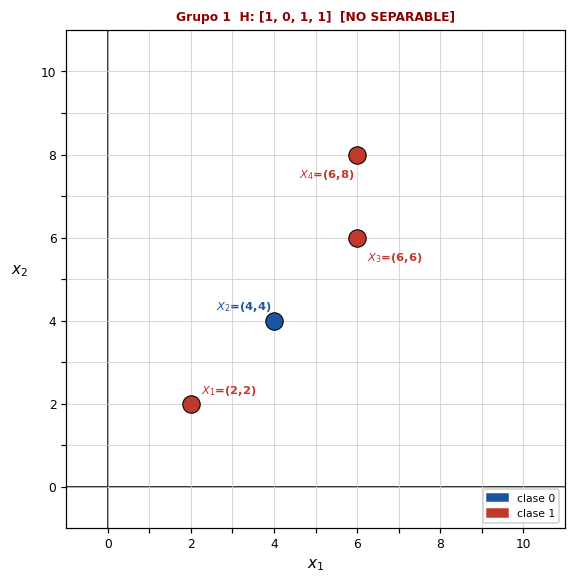
\includegraphics[width=\textwidth]{imagenes_hipotesis/Grupo_1_NS04.png}
    \caption{No separable: [1, 0, 1, 1]}
  \end{subfigure}\hfill
\end{figure}


\section{Grupo 2}
\subsection{Conjunto de puntos}
\begin{table}[H]\centering
  \caption{Coordenadas de Grupo 2}
  \begin{tabular}{ccc}\toprule
    \textbf{Punto} & \textbf{$x_1$} & \textbf{$x_2$}\\\midrule
    $X_{1}$ & 2 & 2 \\
    $X_{2}$ & 2 & 8 \\
    $X_{3}$ & 8 & 2 \\
    $X_{4}$ & 8 & 8 \\
  \bottomrule\end{tabular}
\end{table}

\subsection{Tabla de dic\'otom\'ias ($2^{4}=16$ posibles)}
\begin{table}[H]\centering
  \caption{Todas las dic\'otom\'ias posibles -- Grupo 2}
  \begin{tabular}{cccccc}\toprule
    \textbf{Dic.} & $X_{1}$ & $X_{2}$ & $X_{3}$ & $X_{4}$ & \textbf{Sep.}\\\midrule
    $D_{1}$ & 0 & 0 & 0 & 0 & \textbf{S} \\
    $D_{2}$ & 0 & 0 & 0 & 1 & \textbf{S} \\
    $D_{3}$ & 0 & 0 & 1 & 0 & \textbf{S} \\
    $D_{4}$ & 0 & 0 & 1 & 1 & \textbf{S} \\
    $D_{5}$ & 0 & 1 & 0 & 0 & \textbf{S} \\
    $D_{6}$ & 0 & 1 & 0 & 1 & \textbf{S} \\
    $D_{7}$ & 0 & 1 & 1 & 0 & No \\
    $D_{8}$ & 0 & 1 & 1 & 1 & \textbf{S} \\
    $D_{9}$ & 1 & 0 & 0 & 0 & \textbf{S} \\
    $D_{10}$ & 1 & 0 & 0 & 1 & No \\
    $D_{11}$ & 1 & 0 & 1 & 0 & \textbf{S} \\
    $D_{12}$ & 1 & 0 & 1 & 1 & \textbf{S} \\
    $D_{13}$ & 1 & 1 & 0 & 0 & \textbf{S} \\
    $D_{14}$ & 1 & 1 & 0 & 1 & \textbf{S} \\
    $D_{15}$ & 1 & 1 & 1 & 0 & \textbf{S} \\
    $D_{16}$ & 1 & 1 & 1 & 1 & \textbf{S} \\
  \bottomrule\end{tabular}
\end{table}

\subsection{Hip\'otesis v\'alidas}

\subsubsection{Hip\'otesis $H_{1}$: etiquetas [0, 0, 0, 0]}
\begin{table}[H]\centering
  \caption{Clasificaci\'on de $H_{1}$}
  \begin{tabular}{ccc}\toprule
    \textbf{Punto} & \textbf{Coordenadas} & \textbf{Clase}\\\midrule
    $X_{1}$ & (2, 2) & 0 \\
    $X_{2}$ & (2, 8) & 0 \\
    $X_{3}$ & (8, 2) & 0 \\
    $X_{4}$ & (8, 8) & 0 \\
  \bottomrule\end{tabular}
\end{table}
\begin{figure}[H]\centering
  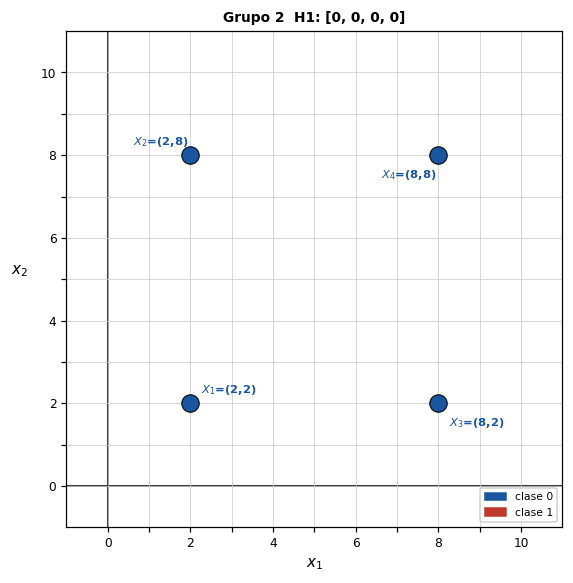
\includegraphics[width=0.65\textwidth]{imagenes_hipotesis/Grupo_2_H01.png}
  \caption{$H_{1}$ -- Grupo 2}
\end{figure}
\textbf{An\'alisis:}
\begin{itemize}
  \item Esta hip\'otesis es \textbf{trivial}: todos los puntos pertenecen a la misma clase.
  \item No existe frontera de decisi\'on expl\'icita.
\end{itemize}

\subsubsection{Hip\'otesis $H_{2}$: etiquetas [0, 0, 0, 1]}
\begin{table}[H]\centering
  \caption{Clasificaci\'on de $H_{2}$}
  \begin{tabular}{ccc}\toprule
    \textbf{Punto} & \textbf{Coordenadas} & \textbf{Clase}\\\midrule
    $X_{1}$ & (2, 2) & 0 \\
    $X_{2}$ & (2, 8) & 0 \\
    $X_{3}$ & (8, 2) & 0 \\
    $X_{4}$ & (8, 8) & 1 \\
  \bottomrule\end{tabular}
\end{table}
\begin{figure}[H]\centering
  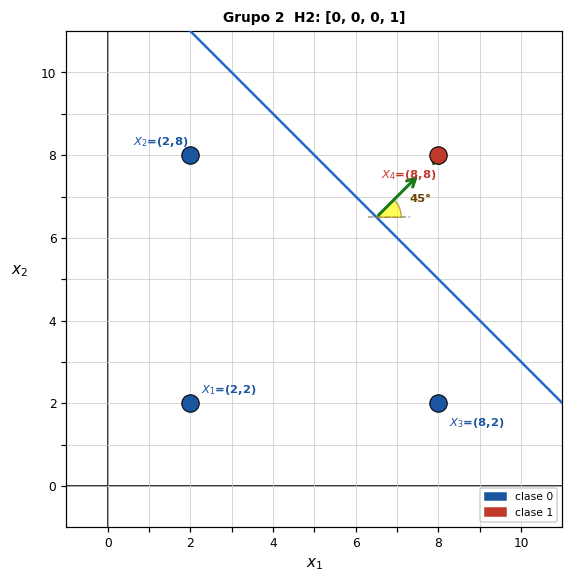
\includegraphics[width=0.65\textwidth]{imagenes_hipotesis/Grupo_2_H02.png}
  \caption{$H_{2}$ -- Grupo 2}
\end{figure}
\textbf{An\'alisis:}
\begin{itemize}
  \item \textbf{Funci\'on separadora:} $0.33 x_1 + 0.33 x_2 - 4.33 = 0$
  \item \textbf{Vector normal:} $\mathbf{w} = (0.333, 0.333)$, perpendicular a la recta.
  \item \textbf{\'Angulo:} $\theta = 45.0 grados$.
  \item \textbf{Direcci\'on de $\mathbf{w}$:} El vector $\mathbf{w}$ apunta hacia el \textbf{cuadrante superior-derecho} ($x_1$ positivo, $x_2$ positivo). La clase~1 se encuentra en esa direcci'on respecto a la frontera.
  \item \textbf{Clase 0} (lado negativo): $X_{1}$, $X_{2}$, $X_{3}$
  \item \textbf{Clase 1} (lado positivo, direcci\'on de $\mathbf{w}$): $X_{4}$
\end{itemize}

\subsubsection{Hip\'otesis $H_{3}$: etiquetas [0, 0, 1, 0]}
\begin{table}[H]\centering
  \caption{Clasificaci\'on de $H_{3}$}
  \begin{tabular}{ccc}\toprule
    \textbf{Punto} & \textbf{Coordenadas} & \textbf{Clase}\\\midrule
    $X_{1}$ & (2, 2) & 0 \\
    $X_{2}$ & (2, 8) & 0 \\
    $X_{3}$ & (8, 2) & 1 \\
    $X_{4}$ & (8, 8) & 0 \\
  \bottomrule\end{tabular}
\end{table}
\begin{figure}[H]\centering
  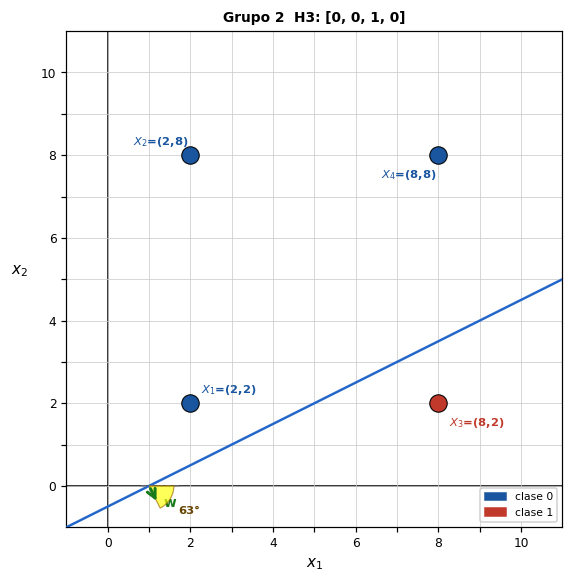
\includegraphics[width=0.65\textwidth]{imagenes_hipotesis/Grupo_2_H03.png}
  \caption{$H_{3}$ -- Grupo 2}
\end{figure}
\textbf{An\'alisis:}
\begin{itemize}
  \item \textbf{Funci\'on separadora:} $0.33 x_1 - 0.67 x_2 - 0.33 = 0$
  \item \textbf{Vector normal:} $\mathbf{w} = (0.333, -0.667)$, perpendicular a la recta.
  \item \textbf{\'Angulo:} $\theta = 296.6 grados$.
  \item \textbf{Direcci\'on de $\mathbf{w}$:} El vector $\mathbf{w}$ apunta hacia el \textbf{cuadrante inferior-derecho} ($x_1$ positivo, $x_2$ negativo). La clase~1 se encuentra en la regi'on inferior-derecha.
  \item \textbf{Clase 0} (lado negativo): $X_{1}$, $X_{2}$, $X_{4}$
  \item \textbf{Clase 1} (lado positivo, direcci\'on de $\mathbf{w}$): $X_{3}$
\end{itemize}

\subsubsection{Hip\'otesis $H_{4}$: etiquetas [0, 0, 1, 1]}
\begin{table}[H]\centering
  \caption{Clasificaci\'on de $H_{4}$}
  \begin{tabular}{ccc}\toprule
    \textbf{Punto} & \textbf{Coordenadas} & \textbf{Clase}\\\midrule
    $X_{1}$ & (2, 2) & 0 \\
    $X_{2}$ & (2, 8) & 0 \\
    $X_{3}$ & (8, 2) & 1 \\
    $X_{4}$ & (8, 8) & 1 \\
  \bottomrule\end{tabular}
\end{table}
\begin{figure}[H]\centering
  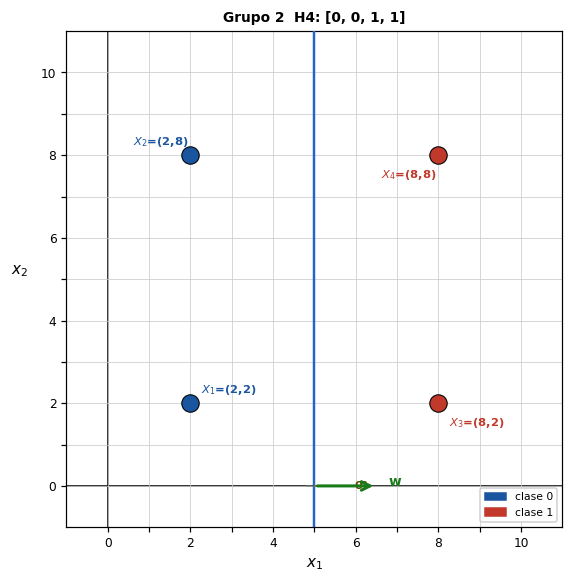
\includegraphics[width=0.65\textwidth]{imagenes_hipotesis/Grupo_2_H04.png}
  \caption{$H_{4}$ -- Grupo 2}
\end{figure}
\textbf{An\'alisis:}
\begin{itemize}
  \item \textbf{Funci\'on separadora:} $0.33 x_1 - 0.00 x_2 - 1.67 = 0$
  \item \textbf{Vector normal:} $\mathbf{w} = (0.333, -0.000)$, perpendicular a la recta.
  \item \textbf{\'Angulo:} $\theta = 360.0 grados$.
  \item \textbf{Direcci\'on de $\mathbf{w}$:} El vector $\mathbf{w}$ apunta hacia el \textbf{cuadrante inferior-derecho} ($x_1$ positivo, $x_2$ negativo). La clase~1 se encuentra en la regi'on inferior-derecha.
  \item \textbf{Clase 0} (lado negativo): $X_{1}$, $X_{2}$
  \item \textbf{Clase 1} (lado positivo, direcci\'on de $\mathbf{w}$): $X_{3}$, $X_{4}$
\end{itemize}

\subsubsection{Hip\'otesis $H_{5}$: etiquetas [0, 1, 0, 0]}
\begin{table}[H]\centering
  \caption{Clasificaci\'on de $H_{5}$}
  \begin{tabular}{ccc}\toprule
    \textbf{Punto} & \textbf{Coordenadas} & \textbf{Clase}\\\midrule
    $X_{1}$ & (2, 2) & 0 \\
    $X_{2}$ & (2, 8) & 1 \\
    $X_{3}$ & (8, 2) & 0 \\
    $X_{4}$ & (8, 8) & 0 \\
  \bottomrule\end{tabular}
\end{table}
\begin{figure}[H]\centering
  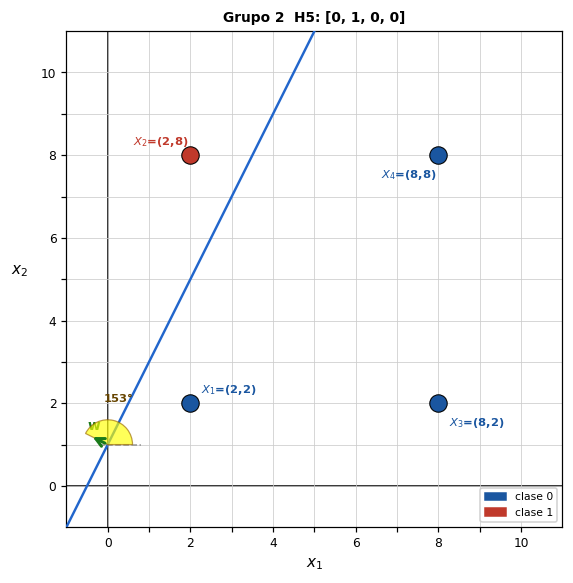
\includegraphics[width=0.65\textwidth]{imagenes_hipotesis/Grupo_2_H05.png}
  \caption{$H_{5}$ -- Grupo 2}
\end{figure}
\textbf{An\'alisis:}
\begin{itemize}
  \item \textbf{Funci\'on separadora:} $-0.67 x_1 + 0.33 x_2 - 0.33 = 0$
  \item \textbf{Vector normal:} $\mathbf{w} = (-0.667, 0.333)$, perpendicular a la recta.
  \item \textbf{\'Angulo:} $\theta = 153.4 grados$.
  \item \textbf{Direcci\'on de $\mathbf{w}$:} El vector $\mathbf{w}$ apunta hacia el \textbf{cuadrante superior-izquierdo} ($x_1$ negativo, $x_2$ positivo). La clase~1 se encuentra a la izquierda y arriba de la frontera.
  \item \textbf{Clase 0} (lado negativo): $X_{1}$, $X_{3}$, $X_{4}$
  \item \textbf{Clase 1} (lado positivo, direcci\'on de $\mathbf{w}$): $X_{2}$
\end{itemize}

\subsubsection{Hip\'otesis $H_{6}$: etiquetas [0, 1, 0, 1]}
\begin{table}[H]\centering
  \caption{Clasificaci\'on de $H_{6}$}
  \begin{tabular}{ccc}\toprule
    \textbf{Punto} & \textbf{Coordenadas} & \textbf{Clase}\\\midrule
    $X_{1}$ & (2, 2) & 0 \\
    $X_{2}$ & (2, 8) & 1 \\
    $X_{3}$ & (8, 2) & 0 \\
    $X_{4}$ & (8, 8) & 1 \\
  \bottomrule\end{tabular}
\end{table}
\begin{figure}[H]\centering
  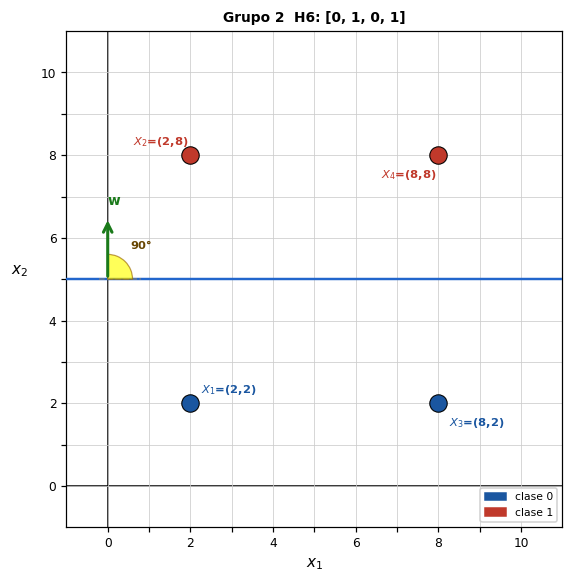
\includegraphics[width=0.65\textwidth]{imagenes_hipotesis/Grupo_2_H06.png}
  \caption{$H_{6}$ -- Grupo 2}
\end{figure}
\textbf{An\'alisis:}
\begin{itemize}
  \item \textbf{Funci\'on separadora:} $-0.00 x_1 + 0.33 x_2 - 1.67 = 0$
  \item \textbf{Vector normal:} $\mathbf{w} = (-0.000, 0.333)$, perpendicular a la recta.
  \item \textbf{\'Angulo:} $\theta = 90.0 grados$.
  \item \textbf{Direcci\'on de $\mathbf{w}$:} El vector $\mathbf{w}$ apunta hacia el \textbf{cuadrante superior-izquierdo} ($x_1$ negativo, $x_2$ positivo). La clase~1 se encuentra a la izquierda y arriba de la frontera.
  \item \textbf{Clase 0} (lado negativo): $X_{1}$, $X_{3}$
  \item \textbf{Clase 1} (lado positivo, direcci\'on de $\mathbf{w}$): $X_{2}$, $X_{4}$
\end{itemize}

\subsubsection{Hip\'otesis $H_{7}$: etiquetas [0, 1, 1, 1]}
\begin{table}[H]\centering
  \caption{Clasificaci\'on de $H_{7}$}
  \begin{tabular}{ccc}\toprule
    \textbf{Punto} & \textbf{Coordenadas} & \textbf{Clase}\\\midrule
    $X_{1}$ & (2, 2) & 0 \\
    $X_{2}$ & (2, 8) & 1 \\
    $X_{3}$ & (8, 2) & 1 \\
    $X_{4}$ & (8, 8) & 1 \\
  \bottomrule\end{tabular}
\end{table}
\begin{figure}[H]\centering
  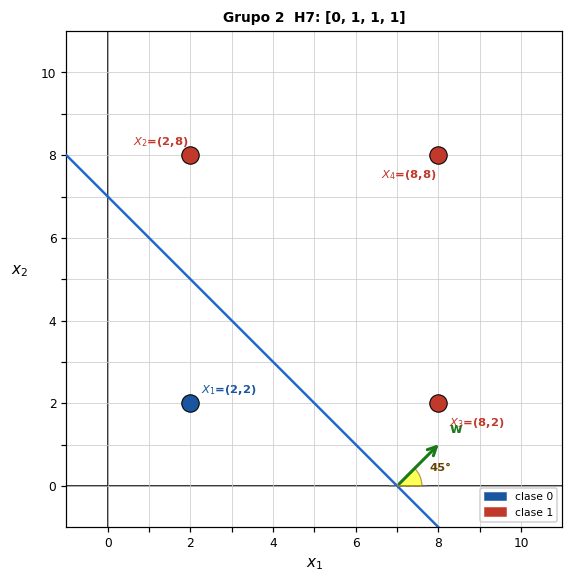
\includegraphics[width=0.65\textwidth]{imagenes_hipotesis/Grupo_2_H07.png}
  \caption{$H_{7}$ -- Grupo 2}
\end{figure}
\textbf{An\'alisis:}
\begin{itemize}
  \item \textbf{Funci\'on separadora:} $0.33 x_1 + 0.33 x_2 - 2.33 = 0$
  \item \textbf{Vector normal:} $\mathbf{w} = (0.333, 0.333)$, perpendicular a la recta.
  \item \textbf{\'Angulo:} $\theta = 45.0 grados$.
  \item \textbf{Direcci\'on de $\mathbf{w}$:} El vector $\mathbf{w}$ apunta hacia el \textbf{cuadrante superior-derecho} ($x_1$ positivo, $x_2$ positivo). La clase~1 se encuentra en esa direcci'on respecto a la frontera.
  \item \textbf{Clase 0} (lado negativo): $X_{1}$
  \item \textbf{Clase 1} (lado positivo, direcci\'on de $\mathbf{w}$): $X_{2}$, $X_{3}$, $X_{4}$
\end{itemize}

\subsubsection{Hip\'otesis $H_{8}$: etiquetas [1, 0, 0, 0]}
\begin{table}[H]\centering
  \caption{Clasificaci\'on de $H_{8}$}
  \begin{tabular}{ccc}\toprule
    \textbf{Punto} & \textbf{Coordenadas} & \textbf{Clase}\\\midrule
    $X_{1}$ & (2, 2) & 1 \\
    $X_{2}$ & (2, 8) & 0 \\
    $X_{3}$ & (8, 2) & 0 \\
    $X_{4}$ & (8, 8) & 0 \\
  \bottomrule\end{tabular}
\end{table}
\begin{figure}[H]\centering
  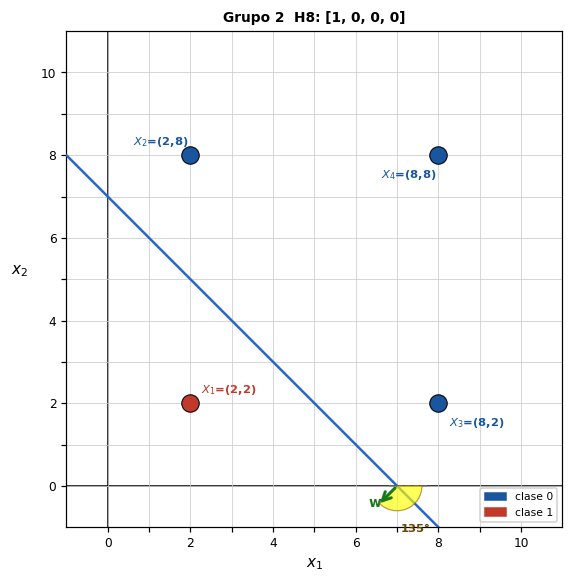
\includegraphics[width=0.65\textwidth]{imagenes_hipotesis/Grupo_2_H08.png}
  \caption{$H_{8}$ -- Grupo 2}
\end{figure}
\textbf{An\'alisis:}
\begin{itemize}
  \item \textbf{Funci\'on separadora:} $-0.33 x_1 - 0.33 x_2 + 2.33 = 0$
  \item \textbf{Vector normal:} $\mathbf{w} = (-0.333, -0.333)$, perpendicular a la recta.
  \item \textbf{\'Angulo:} $\theta = 225.0 grados$.
  \item \textbf{Direcci\'on de $\mathbf{w}$:} El vector $\mathbf{w}$ apunta hacia el \textbf{cuadrante inferior-izquierdo} ($x_1$ negativo, $x_2$ negativo). La clase~1 se encuentra en la regi'on inferior-izquierda.
  \item \textbf{Clase 0} (lado negativo): $X_{2}$, $X_{3}$, $X_{4}$
  \item \textbf{Clase 1} (lado positivo, direcci\'on de $\mathbf{w}$): $X_{1}$
\end{itemize}

\subsubsection{Hip\'otesis $H_{9}$: etiquetas [1, 0, 1, 0]}
\begin{table}[H]\centering
  \caption{Clasificaci\'on de $H_{9}$}
  \begin{tabular}{ccc}\toprule
    \textbf{Punto} & \textbf{Coordenadas} & \textbf{Clase}\\\midrule
    $X_{1}$ & (2, 2) & 1 \\
    $X_{2}$ & (2, 8) & 0 \\
    $X_{3}$ & (8, 2) & 1 \\
    $X_{4}$ & (8, 8) & 0 \\
  \bottomrule\end{tabular}
\end{table}
\begin{figure}[H]\centering
  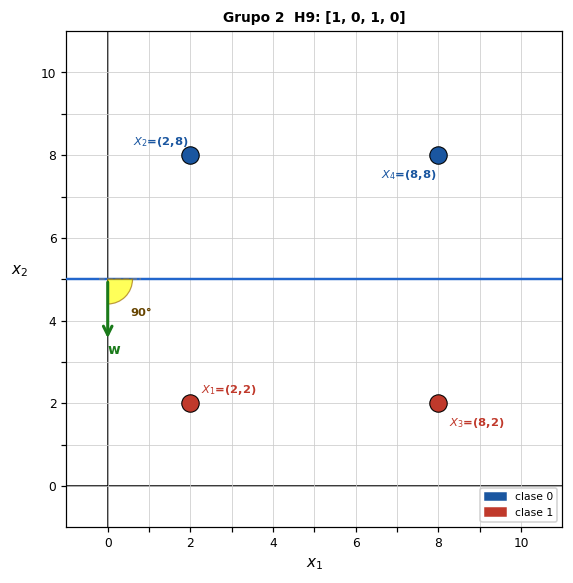
\includegraphics[width=0.65\textwidth]{imagenes_hipotesis/Grupo_2_H09.png}
  \caption{$H_{9}$ -- Grupo 2}
\end{figure}
\textbf{An\'alisis:}
\begin{itemize}
  \item \textbf{Funci\'on separadora:} $0.00 x_1 - 0.33 x_2 + 1.67 = 0$
  \item \textbf{Vector normal:} $\mathbf{w} = (0.000, -0.333)$, perpendicular a la recta.
  \item \textbf{\'Angulo:} $\theta = 270.0 grados$.
  \item \textbf{Direcci\'on de $\mathbf{w}$:} El vector $\mathbf{w}$ apunta hacia el \textbf{cuadrante inferior-derecho} ($x_1$ positivo, $x_2$ negativo). La clase~1 se encuentra en la regi'on inferior-derecha.
  \item \textbf{Clase 0} (lado negativo): $X_{2}$, $X_{4}$
  \item \textbf{Clase 1} (lado positivo, direcci\'on de $\mathbf{w}$): $X_{1}$, $X_{3}$
\end{itemize}

\subsubsection{Hip\'otesis $H_{10}$: etiquetas [1, 0, 1, 1]}
\begin{table}[H]\centering
  \caption{Clasificaci\'on de $H_{10}$}
  \begin{tabular}{ccc}\toprule
    \textbf{Punto} & \textbf{Coordenadas} & \textbf{Clase}\\\midrule
    $X_{1}$ & (2, 2) & 1 \\
    $X_{2}$ & (2, 8) & 0 \\
    $X_{3}$ & (8, 2) & 1 \\
    $X_{4}$ & (8, 8) & 1 \\
  \bottomrule\end{tabular}
\end{table}
\begin{figure}[H]\centering
  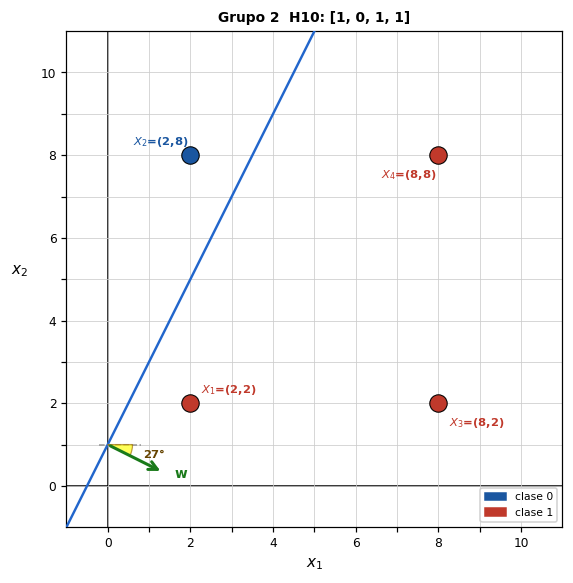
\includegraphics[width=0.65\textwidth]{imagenes_hipotesis/Grupo_2_H10.png}
  \caption{$H_{10}$ -- Grupo 2}
\end{figure}
\textbf{An\'alisis:}
\begin{itemize}
  \item \textbf{Funci\'on separadora:} $0.67 x_1 - 0.33 x_2 + 0.33 = 0$
  \item \textbf{Vector normal:} $\mathbf{w} = (0.667, -0.333)$, perpendicular a la recta.
  \item \textbf{\'Angulo:} $\theta = 333.4 grados$.
  \item \textbf{Direcci\'on de $\mathbf{w}$:} El vector $\mathbf{w}$ apunta hacia el \textbf{cuadrante inferior-derecho} ($x_1$ positivo, $x_2$ negativo). La clase~1 se encuentra en la regi'on inferior-derecha.
  \item \textbf{Clase 0} (lado negativo): $X_{2}$
  \item \textbf{Clase 1} (lado positivo, direcci\'on de $\mathbf{w}$): $X_{1}$, $X_{3}$, $X_{4}$
\end{itemize}

\subsubsection{Hip\'otesis $H_{11}$: etiquetas [1, 1, 0, 0]}
\begin{table}[H]\centering
  \caption{Clasificaci\'on de $H_{11}$}
  \begin{tabular}{ccc}\toprule
    \textbf{Punto} & \textbf{Coordenadas} & \textbf{Clase}\\\midrule
    $X_{1}$ & (2, 2) & 1 \\
    $X_{2}$ & (2, 8) & 1 \\
    $X_{3}$ & (8, 2) & 0 \\
    $X_{4}$ & (8, 8) & 0 \\
  \bottomrule\end{tabular}
\end{table}
\begin{figure}[H]\centering
  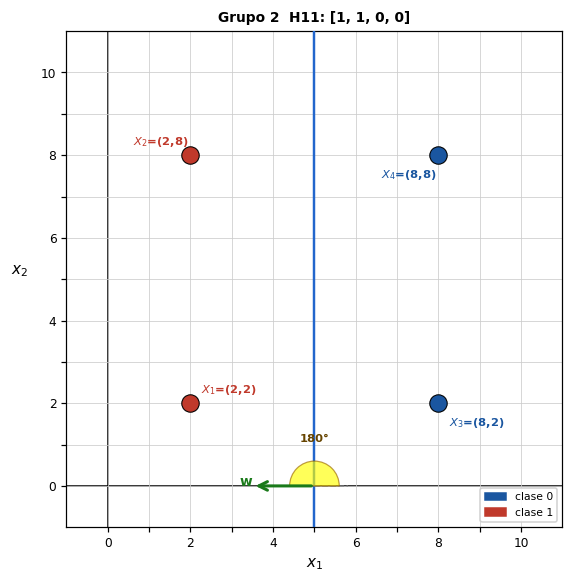
\includegraphics[width=0.65\textwidth]{imagenes_hipotesis/Grupo_2_H11.png}
  \caption{$H_{11}$ -- Grupo 2}
\end{figure}
\textbf{An\'alisis:}
\begin{itemize}
  \item \textbf{Funci\'on separadora:} $-0.33 x_1 + 0.00 x_2 + 1.67 = 0$
  \item \textbf{Vector normal:} $\mathbf{w} = (-0.333, 0.000)$, perpendicular a la recta.
  \item \textbf{\'Angulo:} $\theta = 180.0 grados$.
  \item \textbf{Direcci\'on de $\mathbf{w}$:} El vector $\mathbf{w}$ apunta hacia el \textbf{cuadrante inferior-izquierdo} ($x_1$ negativo, $x_2$ negativo). La clase~1 se encuentra en la regi'on inferior-izquierda.
  \item \textbf{Clase 0} (lado negativo): $X_{3}$, $X_{4}$
  \item \textbf{Clase 1} (lado positivo, direcci\'on de $\mathbf{w}$): $X_{1}$, $X_{2}$
\end{itemize}

\subsubsection{Hip\'otesis $H_{12}$: etiquetas [1, 1, 0, 1]}
\begin{table}[H]\centering
  \caption{Clasificaci\'on de $H_{12}$}
  \begin{tabular}{ccc}\toprule
    \textbf{Punto} & \textbf{Coordenadas} & \textbf{Clase}\\\midrule
    $X_{1}$ & (2, 2) & 1 \\
    $X_{2}$ & (2, 8) & 1 \\
    $X_{3}$ & (8, 2) & 0 \\
    $X_{4}$ & (8, 8) & 1 \\
  \bottomrule\end{tabular}
\end{table}
\begin{figure}[H]\centering
  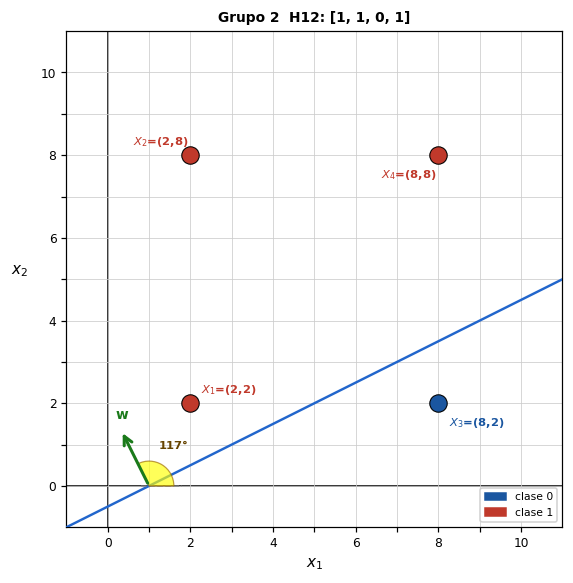
\includegraphics[width=0.65\textwidth]{imagenes_hipotesis/Grupo_2_H12.png}
  \caption{$H_{12}$ -- Grupo 2}
\end{figure}
\textbf{An\'alisis:}
\begin{itemize}
  \item \textbf{Funci\'on separadora:} $-0.33 x_1 + 0.67 x_2 + 0.33 = 0$
  \item \textbf{Vector normal:} $\mathbf{w} = (-0.333, 0.667)$, perpendicular a la recta.
  \item \textbf{\'Angulo:} $\theta = 116.6 grados$.
  \item \textbf{Direcci\'on de $\mathbf{w}$:} El vector $\mathbf{w}$ apunta hacia el \textbf{cuadrante superior-izquierdo} ($x_1$ negativo, $x_2$ positivo). La clase~1 se encuentra a la izquierda y arriba de la frontera.
  \item \textbf{Clase 0} (lado negativo): $X_{3}$
  \item \textbf{Clase 1} (lado positivo, direcci\'on de $\mathbf{w}$): $X_{1}$, $X_{2}$, $X_{4}$
\end{itemize}

\subsubsection{Hip\'otesis $H_{13}$: etiquetas [1, 1, 1, 0]}
\begin{table}[H]\centering
  \caption{Clasificaci\'on de $H_{13}$}
  \begin{tabular}{ccc}\toprule
    \textbf{Punto} & \textbf{Coordenadas} & \textbf{Clase}\\\midrule
    $X_{1}$ & (2, 2) & 1 \\
    $X_{2}$ & (2, 8) & 1 \\
    $X_{3}$ & (8, 2) & 1 \\
    $X_{4}$ & (8, 8) & 0 \\
  \bottomrule\end{tabular}
\end{table}
\begin{figure}[H]\centering
  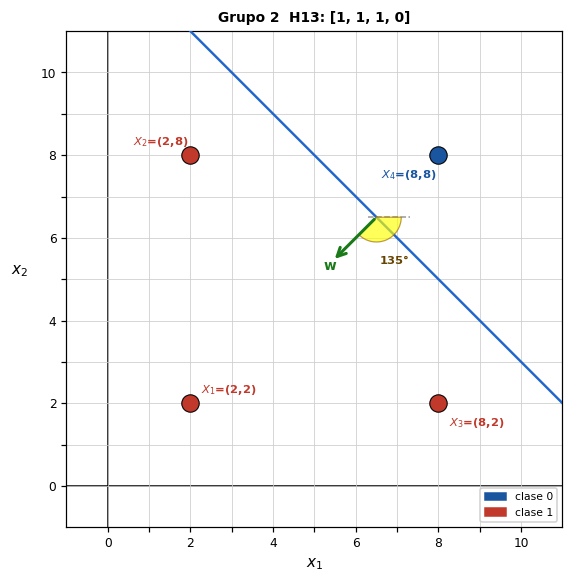
\includegraphics[width=0.65\textwidth]{imagenes_hipotesis/Grupo_2_H13.png}
  \caption{$H_{13}$ -- Grupo 2}
\end{figure}
\textbf{An\'alisis:}
\begin{itemize}
  \item \textbf{Funci\'on separadora:} $-0.33 x_1 - 0.33 x_2 + 4.33 = 0$
  \item \textbf{Vector normal:} $\mathbf{w} = (-0.333, -0.333)$, perpendicular a la recta.
  \item \textbf{\'Angulo:} $\theta = 225.0 grados$.
  \item \textbf{Direcci\'on de $\mathbf{w}$:} El vector $\mathbf{w}$ apunta hacia el \textbf{cuadrante inferior-izquierdo} ($x_1$ negativo, $x_2$ negativo). La clase~1 se encuentra en la regi'on inferior-izquierda.
  \item \textbf{Clase 0} (lado negativo): $X_{4}$
  \item \textbf{Clase 1} (lado positivo, direcci\'on de $\mathbf{w}$): $X_{1}$, $X_{2}$, $X_{3}$
\end{itemize}

\subsubsection{Hip\'otesis $H_{14}$: etiquetas [1, 1, 1, 1]}
\begin{table}[H]\centering
  \caption{Clasificaci\'on de $H_{14}$}
  \begin{tabular}{ccc}\toprule
    \textbf{Punto} & \textbf{Coordenadas} & \textbf{Clase}\\\midrule
    $X_{1}$ & (2, 2) & 1 \\
    $X_{2}$ & (2, 8) & 1 \\
    $X_{3}$ & (8, 2) & 1 \\
    $X_{4}$ & (8, 8) & 1 \\
  \bottomrule\end{tabular}
\end{table}
\begin{figure}[H]\centering
  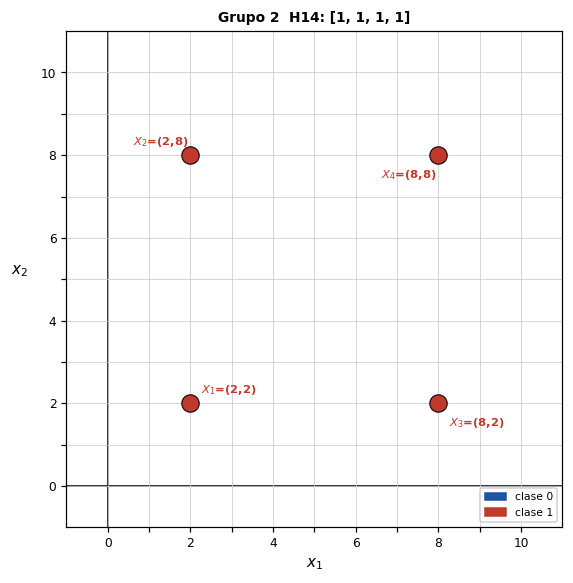
\includegraphics[width=0.65\textwidth]{imagenes_hipotesis/Grupo_2_H14.png}
  \caption{$H_{14}$ -- Grupo 2}
\end{figure}
\textbf{An\'alisis:}
\begin{itemize}
  \item Esta hip\'otesis es \textbf{trivial}: todos los puntos pertenecen a la misma clase.
  \item No existe frontera de decisi\'on expl\'icita.
\end{itemize}

\subsection{Hip\'otesis NO Linealmente Separables}
Las siguientes dic\'otom\'ias \textbf{no pueden ser realizadas}
por ning\'un clasificador lineal sobre este conjunto de puntos.
\begin{figure}[H]\centering
  \begin{subfigure}[b]{0.47\textwidth}
    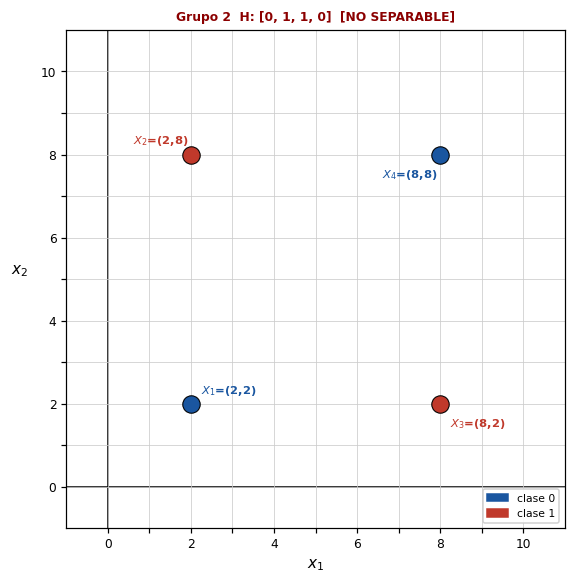
\includegraphics[width=\textwidth]{imagenes_hipotesis/Grupo_2_NS01.png}
    \caption{No separable: [0, 1, 1, 0]}
  \end{subfigure}\hfill
  \begin{subfigure}[b]{0.47\textwidth}
    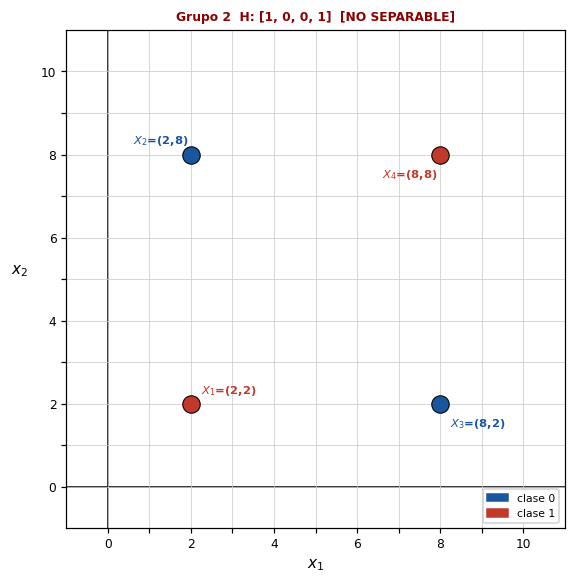
\includegraphics[width=\textwidth]{imagenes_hipotesis/Grupo_2_NS02.png}
    \caption{No separable: [1, 0, 0, 1]}
  \end{subfigure}\hfill
\end{figure}


\section{Grupo 3}
\subsection{Conjunto de puntos}
\begin{table}[H]\centering
  \caption{Coordenadas de Grupo 3}
  \begin{tabular}{ccc}\toprule
    \textbf{Punto} & \textbf{$x_1$} & \textbf{$x_2$}\\\midrule
    $X_{1}$ & 3 & 2 \\
    $X_{2}$ & 5 & 8 \\
    $X_{3}$ & 4 & 6 \\
    $X_{4}$ & 8 & 6 \\
    $X_{5}$ & 7 & 2 \\
  \bottomrule\end{tabular}
\end{table}

\subsection{Tabla de dic\'otom\'ias ($2^{5}=32$ posibles)}
\begin{table}[H]\centering
  \caption{Todas las dic\'otom\'ias posibles -- Grupo 3}
  \begin{tabular}{ccccccc}\toprule
    \textbf{Dic.} & $X_{1}$ & $X_{2}$ & $X_{3}$ & $X_{4}$ & $X_{5}$ & \textbf{Sep.}\\\midrule
    $D_{1}$ & 0 & 0 & 0 & 0 & 0 & \textbf{S} \\
    $D_{2}$ & 0 & 0 & 0 & 0 & 1 & \textbf{S} \\
    $D_{3}$ & 0 & 0 & 0 & 1 & 0 & \textbf{S} \\
    $D_{4}$ & 0 & 0 & 0 & 1 & 1 & \textbf{S} \\
    $D_{5}$ & 0 & 0 & 1 & 0 & 0 & \textbf{S} \\
    $D_{6}$ & 0 & 0 & 1 & 0 & 1 & No \\
    $D_{7}$ & 0 & 0 & 1 & 1 & 0 & No \\
    $D_{8}$ & 0 & 0 & 1 & 1 & 1 & No \\
    $D_{9}$ & 0 & 1 & 0 & 0 & 0 & \textbf{S} \\
    $D_{10}$ & 0 & 1 & 0 & 0 & 1 & No \\
    $D_{11}$ & 0 & 1 & 0 & 1 & 0 & \textbf{S} \\
    $D_{12}$ & 0 & 1 & 0 & 1 & 1 & \textbf{S} \\
    $D_{13}$ & 0 & 1 & 1 & 0 & 0 & \textbf{S} \\
    $D_{14}$ & 0 & 1 & 1 & 0 & 1 & No \\
    $D_{15}$ & 0 & 1 & 1 & 1 & 0 & \textbf{S} \\
    $D_{16}$ & 0 & 1 & 1 & 1 & 1 & \textbf{S} \\
    $D_{17}$ & 1 & 0 & 0 & 0 & 0 & \textbf{S} \\
    $D_{18}$ & 1 & 0 & 0 & 0 & 1 & \textbf{S} \\
    $D_{19}$ & 1 & 0 & 0 & 1 & 0 & No \\
    $D_{20}$ & 1 & 0 & 0 & 1 & 1 & \textbf{S} \\
    $D_{21}$ & 1 & 0 & 1 & 0 & 0 & \textbf{S} \\
    $D_{22}$ & 1 & 0 & 1 & 0 & 1 & \textbf{S} \\
    $D_{23}$ & 1 & 0 & 1 & 1 & 0 & No \\
    $D_{24}$ & 1 & 0 & 1 & 1 & 1 & \textbf{S} \\
    $D_{25}$ & 1 & 1 & 0 & 0 & 0 & No \\
    $D_{26}$ & 1 & 1 & 0 & 0 & 1 & No \\
    $D_{27}$ & 1 & 1 & 0 & 1 & 0 & No \\
    $D_{28}$ & 1 & 1 & 0 & 1 & 1 & \textbf{S} \\
    $D_{29}$ & 1 & 1 & 1 & 0 & 0 & \textbf{S} \\
    $D_{30}$ & 1 & 1 & 1 & 0 & 1 & \textbf{S} \\
    $D_{31}$ & 1 & 1 & 1 & 1 & 0 & \textbf{S} \\
    $D_{32}$ & 1 & 1 & 1 & 1 & 1 & \textbf{S} \\
  \bottomrule\end{tabular}
\end{table}

\subsection{Hip\'otesis v\'alidas}

\subsubsection{Hip\'otesis $H_{1}$: etiquetas [0, 0, 0, 0, 0]}
\begin{table}[H]\centering
  \caption{Clasificaci\'on de $H_{1}$}
  \begin{tabular}{ccc}\toprule
    \textbf{Punto} & \textbf{Coordenadas} & \textbf{Clase}\\\midrule
    $X_{1}$ & (3, 2) & 0 \\
    $X_{2}$ & (5, 8) & 0 \\
    $X_{3}$ & (4, 6) & 0 \\
    $X_{4}$ & (8, 6) & 0 \\
    $X_{5}$ & (7, 2) & 0 \\
  \bottomrule\end{tabular}
\end{table}
\begin{figure}[H]\centering
  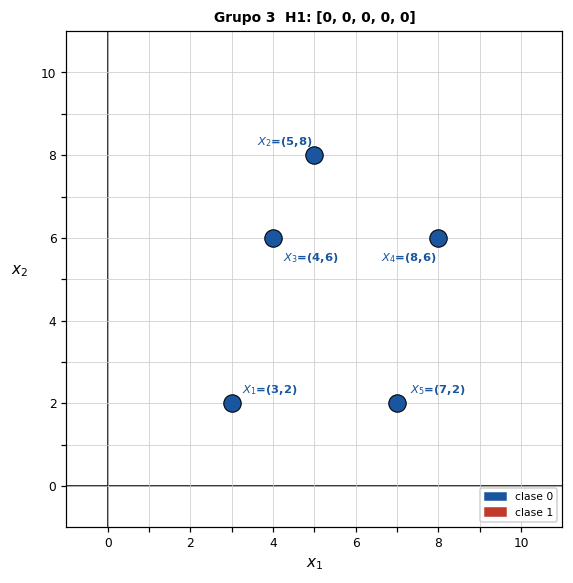
\includegraphics[width=0.65\textwidth]{imagenes_hipotesis/Grupo_3_H01.png}
  \caption{$H_{1}$ -- Grupo 3}
\end{figure}
\textbf{An\'alisis:}
\begin{itemize}
  \item Esta hip\'otesis es \textbf{trivial}: todos los puntos pertenecen a la misma clase.
  \item No existe frontera de decisi\'on expl\'icita.
\end{itemize}

\subsubsection{Hip\'otesis $H_{2}$: etiquetas [0, 0, 0, 0, 1]}
\begin{table}[H]\centering
  \caption{Clasificaci\'on de $H_{2}$}
  \begin{tabular}{ccc}\toprule
    \textbf{Punto} & \textbf{Coordenadas} & \textbf{Clase}\\\midrule
    $X_{1}$ & (3, 2) & 0 \\
    $X_{2}$ & (5, 8) & 0 \\
    $X_{3}$ & (4, 6) & 0 \\
    $X_{4}$ & (8, 6) & 0 \\
    $X_{5}$ & (7, 2) & 1 \\
  \bottomrule\end{tabular}
\end{table}
\begin{figure}[H]\centering
  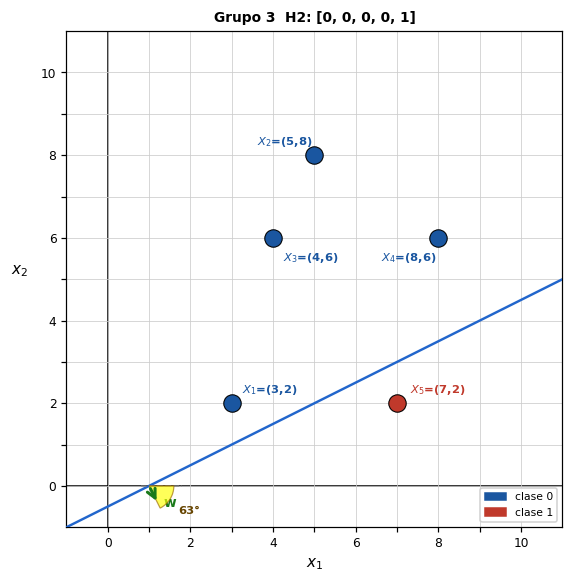
\includegraphics[width=0.65\textwidth]{imagenes_hipotesis/Grupo_3_H02.png}
  \caption{$H_{2}$ -- Grupo 3}
\end{figure}
\textbf{An\'alisis:}
\begin{itemize}
  \item \textbf{Funci\'on separadora:} $0.50 x_1 - 1.00 x_2 - 0.50 = 0$
  \item \textbf{Vector normal:} $\mathbf{w} = (0.500, -1.000)$, perpendicular a la recta.
  \item \textbf{\'Angulo:} $\theta = 296.6 grados$.
  \item \textbf{Direcci\'on de $\mathbf{w}$:} El vector $\mathbf{w}$ apunta hacia el \textbf{cuadrante inferior-derecho} ($x_1$ positivo, $x_2$ negativo). La clase~1 se encuentra en la regi'on inferior-derecha.
  \item \textbf{Clase 0} (lado negativo): $X_{1}$, $X_{2}$, $X_{3}$, $X_{4}$
  \item \textbf{Clase 1} (lado positivo, direcci\'on de $\mathbf{w}$): $X_{5}$
\end{itemize}

\subsubsection{Hip\'otesis $H_{3}$: etiquetas [0, 0, 0, 1, 0]}
\begin{table}[H]\centering
  \caption{Clasificaci\'on de $H_{3}$}
  \begin{tabular}{ccc}\toprule
    \textbf{Punto} & \textbf{Coordenadas} & \textbf{Clase}\\\midrule
    $X_{1}$ & (3, 2) & 0 \\
    $X_{2}$ & (5, 8) & 0 \\
    $X_{3}$ & (4, 6) & 0 \\
    $X_{4}$ & (8, 6) & 1 \\
    $X_{5}$ & (7, 2) & 0 \\
  \bottomrule\end{tabular}
\end{table}
\begin{figure}[H]\centering
  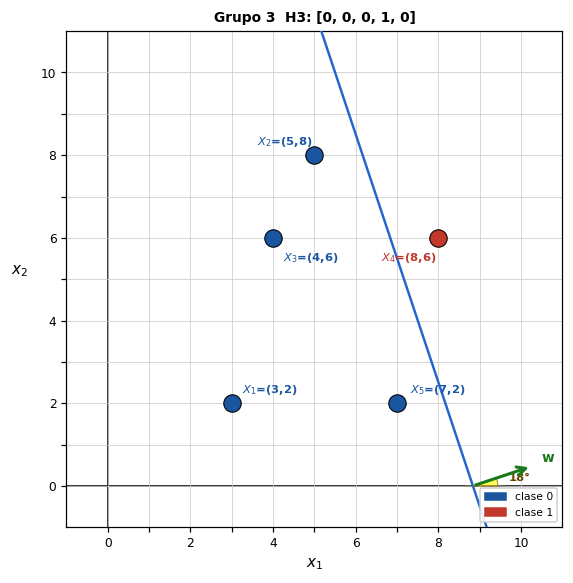
\includegraphics[width=0.65\textwidth]{imagenes_hipotesis/Grupo_3_H03.png}
  \caption{$H_{3}$ -- Grupo 3}
\end{figure}
\textbf{An\'alisis:}
\begin{itemize}
  \item \textbf{Funci\'on separadora:} $0.86 x_1 + 0.29 x_2 - 7.57 = 0$
  \item \textbf{Vector normal:} $\mathbf{w} = (0.857, 0.286)$, perpendicular a la recta.
  \item \textbf{\'Angulo:} $\theta = 18.4 grados$.
  \item \textbf{Direcci\'on de $\mathbf{w}$:} El vector $\mathbf{w}$ apunta hacia el \textbf{cuadrante superior-derecho} ($x_1$ positivo, $x_2$ positivo). La clase~1 se encuentra en esa direcci'on respecto a la frontera.
  \item \textbf{Clase 0} (lado negativo): $X_{1}$, $X_{2}$, $X_{3}$, $X_{5}$
  \item \textbf{Clase 1} (lado positivo, direcci\'on de $\mathbf{w}$): $X_{4}$
\end{itemize}

\subsubsection{Hip\'otesis $H_{4}$: etiquetas [0, 0, 0, 1, 1]}
\begin{table}[H]\centering
  \caption{Clasificaci\'on de $H_{4}$}
  \begin{tabular}{ccc}\toprule
    \textbf{Punto} & \textbf{Coordenadas} & \textbf{Clase}\\\midrule
    $X_{1}$ & (3, 2) & 0 \\
    $X_{2}$ & (5, 8) & 0 \\
    $X_{3}$ & (4, 6) & 0 \\
    $X_{4}$ & (8, 6) & 1 \\
    $X_{5}$ & (7, 2) & 1 \\
  \bottomrule\end{tabular}
\end{table}
\begin{figure}[H]\centering
  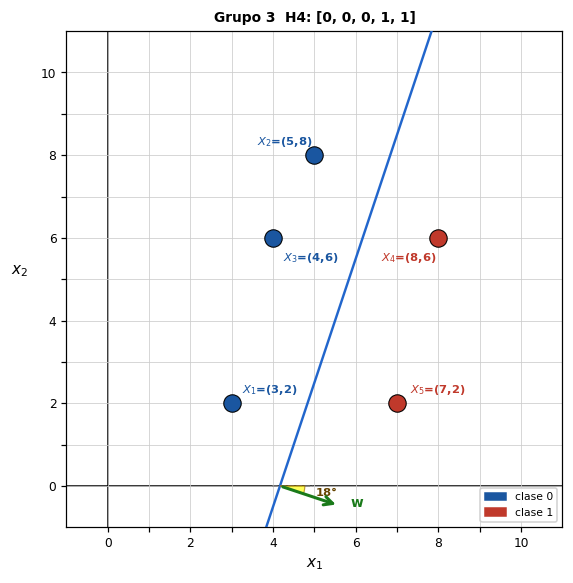
\includegraphics[width=0.65\textwidth]{imagenes_hipotesis/Grupo_3_H04.png}
  \caption{$H_{4}$ -- Grupo 3}
\end{figure}
\textbf{An\'alisis:}
\begin{itemize}
  \item \textbf{Funci\'on separadora:} $0.55 x_1 - 0.18 x_2 - 2.27 = 0$
  \item \textbf{Vector normal:} $\mathbf{w} = (0.545, -0.182)$, perpendicular a la recta.
  \item \textbf{\'Angulo:} $\theta = 341.6 grados$.
  \item \textbf{Direcci\'on de $\mathbf{w}$:} El vector $\mathbf{w}$ apunta hacia el \textbf{cuadrante inferior-derecho} ($x_1$ positivo, $x_2$ negativo). La clase~1 se encuentra en la regi'on inferior-derecha.
  \item \textbf{Clase 0} (lado negativo): $X_{1}$, $X_{2}$, $X_{3}$
  \item \textbf{Clase 1} (lado positivo, direcci\'on de $\mathbf{w}$): $X_{4}$, $X_{5}$
\end{itemize}

\subsubsection{Hip\'otesis $H_{5}$: etiquetas [0, 0, 1, 0, 0]}
\begin{table}[H]\centering
  \caption{Clasificaci\'on de $H_{5}$}
  \begin{tabular}{ccc}\toprule
    \textbf{Punto} & \textbf{Coordenadas} & \textbf{Clase}\\\midrule
    $X_{1}$ & (3, 2) & 0 \\
    $X_{2}$ & (5, 8) & 0 \\
    $X_{3}$ & (4, 6) & 1 \\
    $X_{4}$ & (8, 6) & 0 \\
    $X_{5}$ & (7, 2) & 0 \\
  \bottomrule\end{tabular}
\end{table}
\begin{figure}[H]\centering
  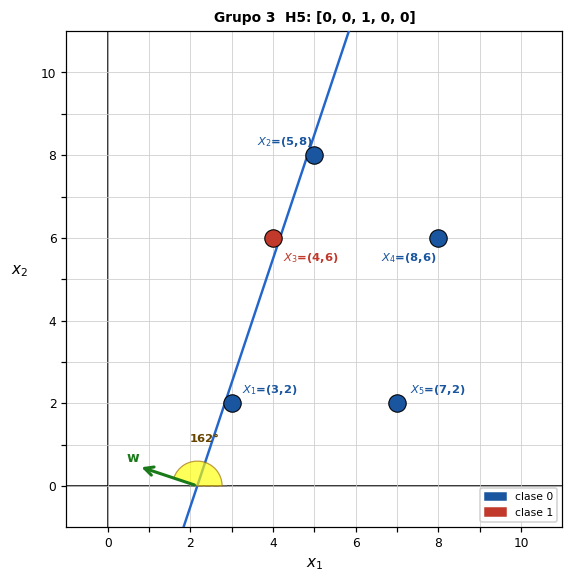
\includegraphics[width=0.65\textwidth]{imagenes_hipotesis/Grupo_3_H05.png}
  \caption{$H_{5}$ -- Grupo 3}
\end{figure}
\textbf{An\'alisis:}
\begin{itemize}
  \item \textbf{Funci\'on separadora:} $-6.00 x_1 + 2.00 x_2 + 13.00 = 0$
  \item \textbf{Vector normal:} $\mathbf{w} = (-6.000, 2.000)$, perpendicular a la recta.
  \item \textbf{\'Angulo:} $\theta = 161.6 grados$.
  \item \textbf{Direcci\'on de $\mathbf{w}$:} El vector $\mathbf{w}$ apunta hacia el \textbf{cuadrante superior-izquierdo} ($x_1$ negativo, $x_2$ positivo). La clase~1 se encuentra a la izquierda y arriba de la frontera.
  \item \textbf{Clase 0} (lado negativo): $X_{1}$, $X_{2}$, $X_{4}$, $X_{5}$
  \item \textbf{Clase 1} (lado positivo, direcci\'on de $\mathbf{w}$): $X_{3}$
\end{itemize}

\subsubsection{Hip\'otesis $H_{6}$: etiquetas [0, 1, 0, 0, 0]}
\begin{table}[H]\centering
  \caption{Clasificaci\'on de $H_{6}$}
  \begin{tabular}{ccc}\toprule
    \textbf{Punto} & \textbf{Coordenadas} & \textbf{Clase}\\\midrule
    $X_{1}$ & (3, 2) & 0 \\
    $X_{2}$ & (5, 8) & 1 \\
    $X_{3}$ & (4, 6) & 0 \\
    $X_{4}$ & (8, 6) & 0 \\
    $X_{5}$ & (7, 2) & 0 \\
  \bottomrule\end{tabular}
\end{table}
\begin{figure}[H]\centering
  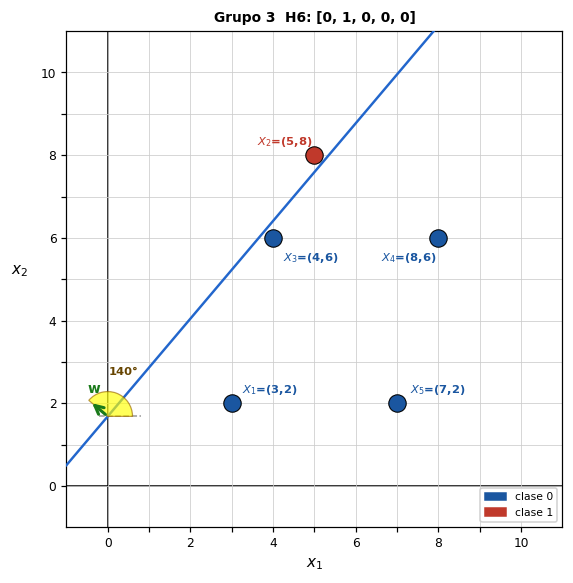
\includegraphics[width=0.65\textwidth]{imagenes_hipotesis/Grupo_3_H06.png}
  \caption{$H_{6}$ -- Grupo 3}
\end{figure}
\textbf{An\'alisis:}
\begin{itemize}
  \item \textbf{Funci\'on separadora:} $-2.89 x_1 + 2.44 x_2 - 4.11 = 0$
  \item \textbf{Vector normal:} $\mathbf{w} = (-2.889, 2.444)$, perpendicular a la recta.
  \item \textbf{\'Angulo:} $\theta = 139.8 grados$.
  \item \textbf{Direcci\'on de $\mathbf{w}$:} El vector $\mathbf{w}$ apunta hacia el \textbf{cuadrante superior-izquierdo} ($x_1$ negativo, $x_2$ positivo). La clase~1 se encuentra a la izquierda y arriba de la frontera.
  \item \textbf{Clase 0} (lado negativo): $X_{1}$, $X_{3}$, $X_{4}$, $X_{5}$
  \item \textbf{Clase 1} (lado positivo, direcci\'on de $\mathbf{w}$): $X_{2}$
\end{itemize}

\subsubsection{Hip\'otesis $H_{7}$: etiquetas [0, 1, 0, 1, 0]}
\begin{table}[H]\centering
  \caption{Clasificaci\'on de $H_{7}$}
  \begin{tabular}{ccc}\toprule
    \textbf{Punto} & \textbf{Coordenadas} & \textbf{Clase}\\\midrule
    $X_{1}$ & (3, 2) & 0 \\
    $X_{2}$ & (5, 8) & 1 \\
    $X_{3}$ & (4, 6) & 0 \\
    $X_{4}$ & (8, 6) & 1 \\
    $X_{5}$ & (7, 2) & 0 \\
  \bottomrule\end{tabular}
\end{table}
\begin{figure}[H]\centering
  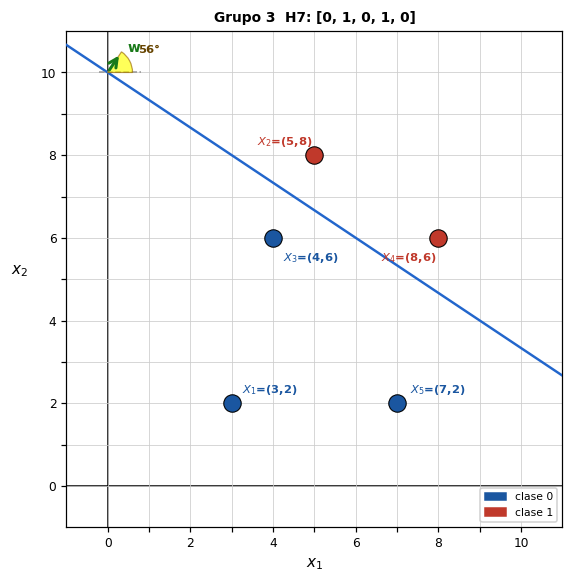
\includegraphics[width=0.65\textwidth]{imagenes_hipotesis/Grupo_3_H07.png}
  \caption{$H_{7}$ -- Grupo 3}
\end{figure}
\textbf{An\'alisis:}
\begin{itemize}
  \item \textbf{Funci\'on separadora:} $0.50 x_1 + 0.75 x_2 - 7.50 = 0$
  \item \textbf{Vector normal:} $\mathbf{w} = (0.500, 0.750)$, perpendicular a la recta.
  \item \textbf{\'Angulo:} $\theta = 56.3 grados$.
  \item \textbf{Direcci\'on de $\mathbf{w}$:} El vector $\mathbf{w}$ apunta hacia el \textbf{cuadrante superior-derecho} ($x_1$ positivo, $x_2$ positivo). La clase~1 se encuentra en esa direcci'on respecto a la frontera.
  \item \textbf{Clase 0} (lado negativo): $X_{1}$, $X_{3}$, $X_{5}$
  \item \textbf{Clase 1} (lado positivo, direcci\'on de $\mathbf{w}$): $X_{2}$, $X_{4}$
\end{itemize}

\subsubsection{Hip\'otesis $H_{8}$: etiquetas [0, 1, 0, 1, 1]}
\begin{table}[H]\centering
  \caption{Clasificaci\'on de $H_{8}$}
  \begin{tabular}{ccc}\toprule
    \textbf{Punto} & \textbf{Coordenadas} & \textbf{Clase}\\\midrule
    $X_{1}$ & (3, 2) & 0 \\
    $X_{2}$ & (5, 8) & 1 \\
    $X_{3}$ & (4, 6) & 0 \\
    $X_{4}$ & (8, 6) & 1 \\
    $X_{5}$ & (7, 2) & 1 \\
  \bottomrule\end{tabular}
\end{table}
\begin{figure}[H]\centering
  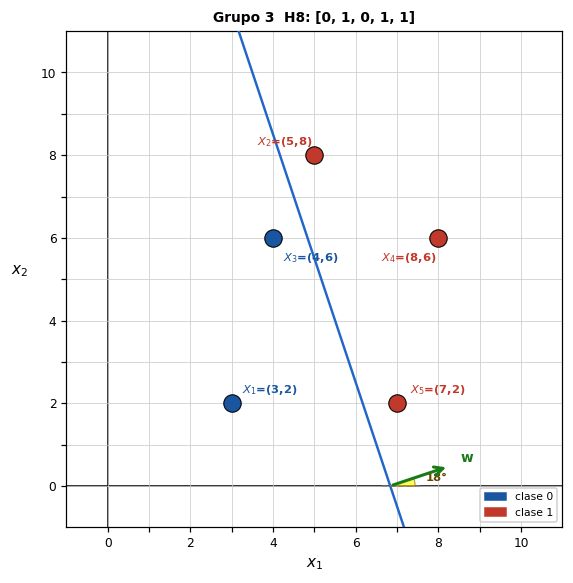
\includegraphics[width=0.65\textwidth]{imagenes_hipotesis/Grupo_3_H08.png}
  \caption{$H_{8}$ -- Grupo 3}
\end{figure}
\textbf{An\'alisis:}
\begin{itemize}
  \item \textbf{Funci\'on separadora:} $1.20 x_1 + 0.40 x_2 - 8.20 = 0$
  \item \textbf{Vector normal:} $\mathbf{w} = (1.200, 0.400)$, perpendicular a la recta.
  \item \textbf{\'Angulo:} $\theta = 18.4 grados$.
  \item \textbf{Direcci\'on de $\mathbf{w}$:} El vector $\mathbf{w}$ apunta hacia el \textbf{cuadrante superior-derecho} ($x_1$ positivo, $x_2$ positivo). La clase~1 se encuentra en esa direcci'on respecto a la frontera.
  \item \textbf{Clase 0} (lado negativo): $X_{1}$, $X_{3}$
  \item \textbf{Clase 1} (lado positivo, direcci\'on de $\mathbf{w}$): $X_{2}$, $X_{4}$, $X_{5}$
\end{itemize}

\subsubsection{Hip\'otesis $H_{9}$: etiquetas [0, 1, 1, 0, 0]}
\begin{table}[H]\centering
  \caption{Clasificaci\'on de $H_{9}$}
  \begin{tabular}{ccc}\toprule
    \textbf{Punto} & \textbf{Coordenadas} & \textbf{Clase}\\\midrule
    $X_{1}$ & (3, 2) & 0 \\
    $X_{2}$ & (5, 8) & 1 \\
    $X_{3}$ & (4, 6) & 1 \\
    $X_{4}$ & (8, 6) & 0 \\
    $X_{5}$ & (7, 2) & 0 \\
  \bottomrule\end{tabular}
\end{table}
\begin{figure}[H]\centering
  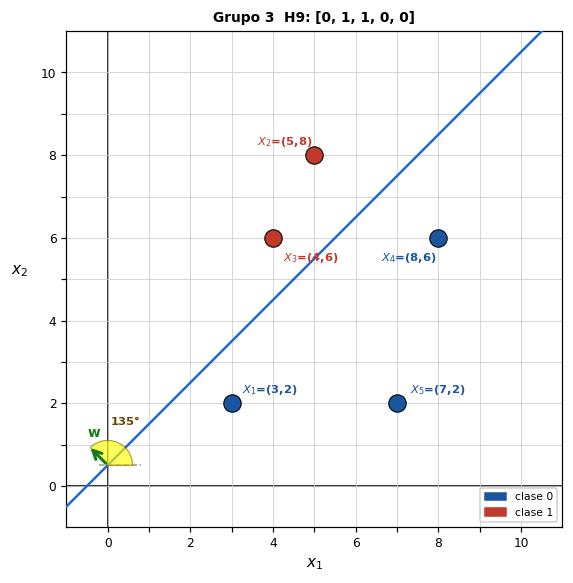
\includegraphics[width=0.65\textwidth]{imagenes_hipotesis/Grupo_3_H09.png}
  \caption{$H_{9}$ -- Grupo 3}
\end{figure}
\textbf{An\'alisis:}
\begin{itemize}
  \item \textbf{Funci\'on separadora:} $-0.67 x_1 + 0.67 x_2 - 0.33 = 0$
  \item \textbf{Vector normal:} $\mathbf{w} = (-0.667, 0.667)$, perpendicular a la recta.
  \item \textbf{\'Angulo:} $\theta = 135.0 grados$.
  \item \textbf{Direcci\'on de $\mathbf{w}$:} El vector $\mathbf{w}$ apunta hacia el \textbf{cuadrante superior-izquierdo} ($x_1$ negativo, $x_2$ positivo). La clase~1 se encuentra a la izquierda y arriba de la frontera.
  \item \textbf{Clase 0} (lado negativo): $X_{1}$, $X_{4}$, $X_{5}$
  \item \textbf{Clase 1} (lado positivo, direcci\'on de $\mathbf{w}$): $X_{2}$, $X_{3}$
\end{itemize}

\subsubsection{Hip\'otesis $H_{10}$: etiquetas [0, 1, 1, 1, 0]}
\begin{table}[H]\centering
  \caption{Clasificaci\'on de $H_{10}$}
  \begin{tabular}{ccc}\toprule
    \textbf{Punto} & \textbf{Coordenadas} & \textbf{Clase}\\\midrule
    $X_{1}$ & (3, 2) & 0 \\
    $X_{2}$ & (5, 8) & 1 \\
    $X_{3}$ & (4, 6) & 1 \\
    $X_{4}$ & (8, 6) & 1 \\
    $X_{5}$ & (7, 2) & 0 \\
  \bottomrule\end{tabular}
\end{table}
\begin{figure}[H]\centering
  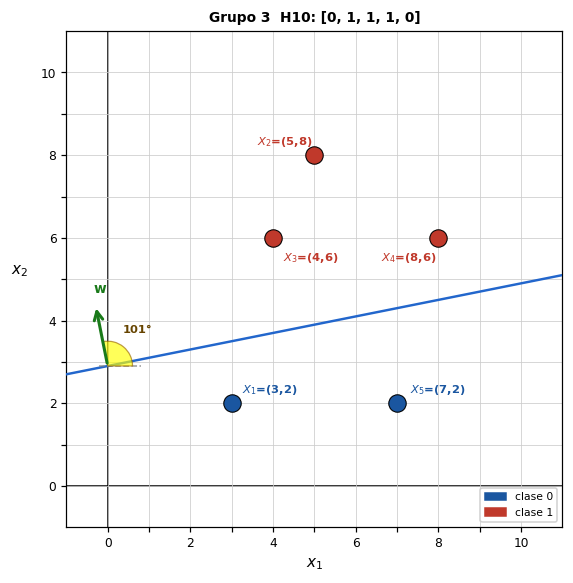
\includegraphics[width=0.65\textwidth]{imagenes_hipotesis/Grupo_3_H10.png}
  \caption{$H_{10}$ -- Grupo 3}
\end{figure}
\textbf{An\'alisis:}
\begin{itemize}
  \item \textbf{Funci\'on separadora:} $-0.13 x_1 + 0.67 x_2 - 1.93 = 0$
  \item \textbf{Vector normal:} $\mathbf{w} = (-0.133, 0.667)$, perpendicular a la recta.
  \item \textbf{\'Angulo:} $\theta = 101.3 grados$.
  \item \textbf{Direcci\'on de $\mathbf{w}$:} El vector $\mathbf{w}$ apunta hacia el \textbf{cuadrante superior-izquierdo} ($x_1$ negativo, $x_2$ positivo). La clase~1 se encuentra a la izquierda y arriba de la frontera.
  \item \textbf{Clase 0} (lado negativo): $X_{1}$, $X_{5}$
  \item \textbf{Clase 1} (lado positivo, direcci\'on de $\mathbf{w}$): $X_{2}$, $X_{3}$, $X_{4}$
\end{itemize}

\subsubsection{Hip\'otesis $H_{11}$: etiquetas [0, 1, 1, 1, 1]}
\begin{table}[H]\centering
  \caption{Clasificaci\'on de $H_{11}$}
  \begin{tabular}{ccc}\toprule
    \textbf{Punto} & \textbf{Coordenadas} & \textbf{Clase}\\\midrule
    $X_{1}$ & (3, 2) & 0 \\
    $X_{2}$ & (5, 8) & 1 \\
    $X_{3}$ & (4, 6) & 1 \\
    $X_{4}$ & (8, 6) & 1 \\
    $X_{5}$ & (7, 2) & 1 \\
  \bottomrule\end{tabular}
\end{table}
\begin{figure}[H]\centering
  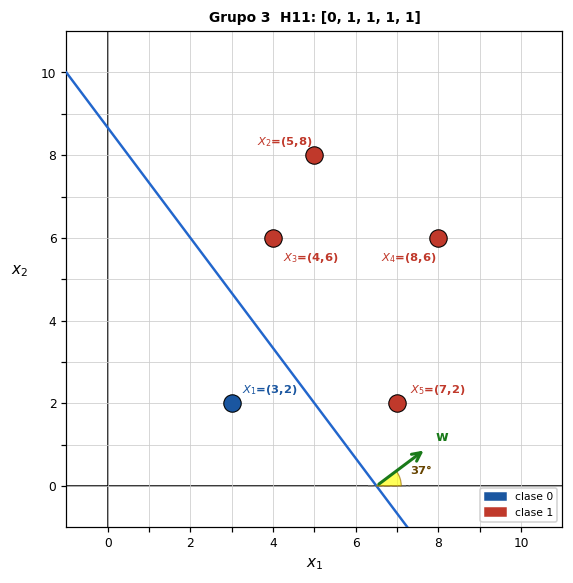
\includegraphics[width=0.65\textwidth]{imagenes_hipotesis/Grupo_3_H11.png}
  \caption{$H_{11}$ -- Grupo 3}
\end{figure}
\textbf{An\'alisis:}
\begin{itemize}
  \item \textbf{Funci\'on separadora:} $0.50 x_1 + 0.37 x_2 - 3.25 = 0$
  \item \textbf{Vector normal:} $\mathbf{w} = (0.500, 0.375)$, perpendicular a la recta.
  \item \textbf{\'Angulo:} $\theta = 36.9 grados$.
  \item \textbf{Direcci\'on de $\mathbf{w}$:} El vector $\mathbf{w}$ apunta hacia el \textbf{cuadrante superior-derecho} ($x_1$ positivo, $x_2$ positivo). La clase~1 se encuentra en esa direcci'on respecto a la frontera.
  \item \textbf{Clase 0} (lado negativo): $X_{1}$
  \item \textbf{Clase 1} (lado positivo, direcci\'on de $\mathbf{w}$): $X_{2}$, $X_{3}$, $X_{4}$, $X_{5}$
\end{itemize}

\subsubsection{Hip\'otesis $H_{12}$: etiquetas [1, 0, 0, 0, 0]}
\begin{table}[H]\centering
  \caption{Clasificaci\'on de $H_{12}$}
  \begin{tabular}{ccc}\toprule
    \textbf{Punto} & \textbf{Coordenadas} & \textbf{Clase}\\\midrule
    $X_{1}$ & (3, 2) & 1 \\
    $X_{2}$ & (5, 8) & 0 \\
    $X_{3}$ & (4, 6) & 0 \\
    $X_{4}$ & (8, 6) & 0 \\
    $X_{5}$ & (7, 2) & 0 \\
  \bottomrule\end{tabular}
\end{table}
\begin{figure}[H]\centering
  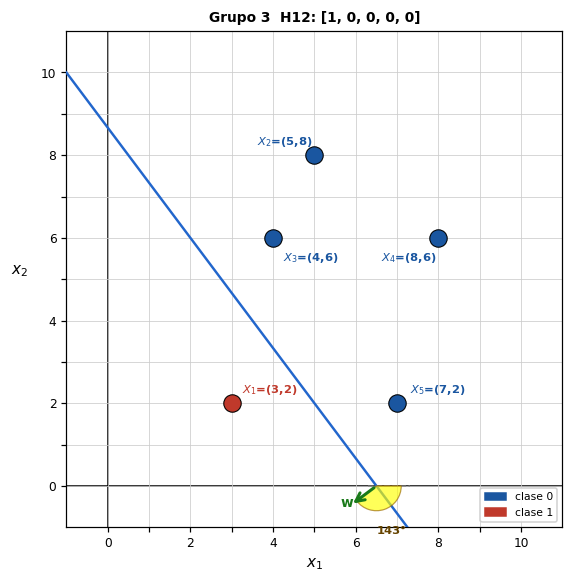
\includegraphics[width=0.65\textwidth]{imagenes_hipotesis/Grupo_3_H12.png}
  \caption{$H_{12}$ -- Grupo 3}
\end{figure}
\textbf{An\'alisis:}
\begin{itemize}
  \item \textbf{Funci\'on separadora:} $-0.50 x_1 - 0.37 x_2 + 3.25 = 0$
  \item \textbf{Vector normal:} $\mathbf{w} = (-0.500, -0.375)$, perpendicular a la recta.
  \item \textbf{\'Angulo:} $\theta = 216.9 grados$.
  \item \textbf{Direcci\'on de $\mathbf{w}$:} El vector $\mathbf{w}$ apunta hacia el \textbf{cuadrante inferior-izquierdo} ($x_1$ negativo, $x_2$ negativo). La clase~1 se encuentra en la regi'on inferior-izquierda.
  \item \textbf{Clase 0} (lado negativo): $X_{2}$, $X_{3}$, $X_{4}$, $X_{5}$
  \item \textbf{Clase 1} (lado positivo, direcci\'on de $\mathbf{w}$): $X_{1}$
\end{itemize}

\subsubsection{Hip\'otesis $H_{13}$: etiquetas [1, 0, 0, 0, 1]}
\begin{table}[H]\centering
  \caption{Clasificaci\'on de $H_{13}$}
  \begin{tabular}{ccc}\toprule
    \textbf{Punto} & \textbf{Coordenadas} & \textbf{Clase}\\\midrule
    $X_{1}$ & (3, 2) & 1 \\
    $X_{2}$ & (5, 8) & 0 \\
    $X_{3}$ & (4, 6) & 0 \\
    $X_{4}$ & (8, 6) & 0 \\
    $X_{5}$ & (7, 2) & 1 \\
  \bottomrule\end{tabular}
\end{table}
\begin{figure}[H]\centering
  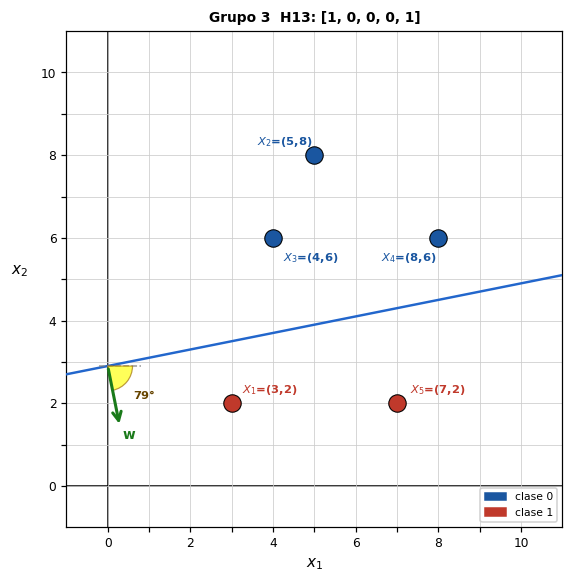
\includegraphics[width=0.65\textwidth]{imagenes_hipotesis/Grupo_3_H13.png}
  \caption{$H_{13}$ -- Grupo 3}
\end{figure}
\textbf{An\'alisis:}
\begin{itemize}
  \item \textbf{Funci\'on separadora:} $0.13 x_1 - 0.67 x_2 + 1.93 = 0$
  \item \textbf{Vector normal:} $\mathbf{w} = (0.133, -0.667)$, perpendicular a la recta.
  \item \textbf{\'Angulo:} $\theta = 281.3 grados$.
  \item \textbf{Direcci\'on de $\mathbf{w}$:} El vector $\mathbf{w}$ apunta hacia el \textbf{cuadrante inferior-derecho} ($x_1$ positivo, $x_2$ negativo). La clase~1 se encuentra en la regi'on inferior-derecha.
  \item \textbf{Clase 0} (lado negativo): $X_{2}$, $X_{3}$, $X_{4}$
  \item \textbf{Clase 1} (lado positivo, direcci\'on de $\mathbf{w}$): $X_{1}$, $X_{5}$
\end{itemize}

\subsubsection{Hip\'otesis $H_{14}$: etiquetas [1, 0, 0, 1, 1]}
\begin{table}[H]\centering
  \caption{Clasificaci\'on de $H_{14}$}
  \begin{tabular}{ccc}\toprule
    \textbf{Punto} & \textbf{Coordenadas} & \textbf{Clase}\\\midrule
    $X_{1}$ & (3, 2) & 1 \\
    $X_{2}$ & (5, 8) & 0 \\
    $X_{3}$ & (4, 6) & 0 \\
    $X_{4}$ & (8, 6) & 1 \\
    $X_{5}$ & (7, 2) & 1 \\
  \bottomrule\end{tabular}
\end{table}
\begin{figure}[H]\centering
  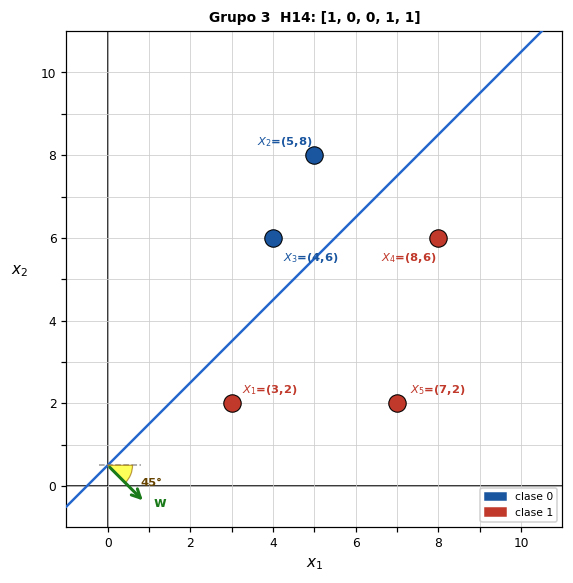
\includegraphics[width=0.65\textwidth]{imagenes_hipotesis/Grupo_3_H14.png}
  \caption{$H_{14}$ -- Grupo 3}
\end{figure}
\textbf{An\'alisis:}
\begin{itemize}
  \item \textbf{Funci\'on separadora:} $0.67 x_1 - 0.67 x_2 + 0.33 = 0$
  \item \textbf{Vector normal:} $\mathbf{w} = (0.667, -0.667)$, perpendicular a la recta.
  \item \textbf{\'Angulo:} $\theta = 315.0 grados$.
  \item \textbf{Direcci\'on de $\mathbf{w}$:} El vector $\mathbf{w}$ apunta hacia el \textbf{cuadrante inferior-derecho} ($x_1$ positivo, $x_2$ negativo). La clase~1 se encuentra en la regi'on inferior-derecha.
  \item \textbf{Clase 0} (lado negativo): $X_{2}$, $X_{3}$
  \item \textbf{Clase 1} (lado positivo, direcci\'on de $\mathbf{w}$): $X_{1}$, $X_{4}$, $X_{5}$
\end{itemize}

\subsubsection{Hip\'otesis $H_{15}$: etiquetas [1, 0, 1, 0, 0]}
\begin{table}[H]\centering
  \caption{Clasificaci\'on de $H_{15}$}
  \begin{tabular}{ccc}\toprule
    \textbf{Punto} & \textbf{Coordenadas} & \textbf{Clase}\\\midrule
    $X_{1}$ & (3, 2) & 1 \\
    $X_{2}$ & (5, 8) & 0 \\
    $X_{3}$ & (4, 6) & 1 \\
    $X_{4}$ & (8, 6) & 0 \\
    $X_{5}$ & (7, 2) & 0 \\
  \bottomrule\end{tabular}
\end{table}
\begin{figure}[H]\centering
  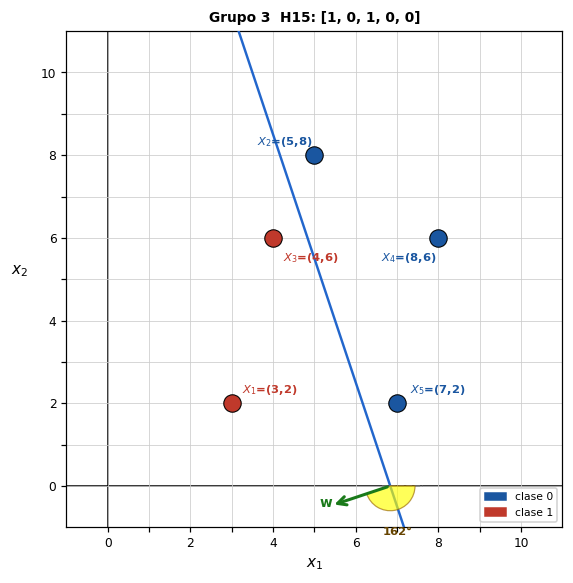
\includegraphics[width=0.65\textwidth]{imagenes_hipotesis/Grupo_3_H15.png}
  \caption{$H_{15}$ -- Grupo 3}
\end{figure}
\textbf{An\'alisis:}
\begin{itemize}
  \item \textbf{Funci\'on separadora:} $-1.20 x_1 - 0.40 x_2 + 8.20 = 0$
  \item \textbf{Vector normal:} $\mathbf{w} = (-1.200, -0.400)$, perpendicular a la recta.
  \item \textbf{\'Angulo:} $\theta = 198.4 grados$.
  \item \textbf{Direcci\'on de $\mathbf{w}$:} El vector $\mathbf{w}$ apunta hacia el \textbf{cuadrante inferior-izquierdo} ($x_1$ negativo, $x_2$ negativo). La clase~1 se encuentra en la regi'on inferior-izquierda.
  \item \textbf{Clase 0} (lado negativo): $X_{2}$, $X_{4}$, $X_{5}$
  \item \textbf{Clase 1} (lado positivo, direcci\'on de $\mathbf{w}$): $X_{1}$, $X_{3}$
\end{itemize}

\subsubsection{Hip\'otesis $H_{16}$: etiquetas [1, 0, 1, 0, 1]}
\begin{table}[H]\centering
  \caption{Clasificaci\'on de $H_{16}$}
  \begin{tabular}{ccc}\toprule
    \textbf{Punto} & \textbf{Coordenadas} & \textbf{Clase}\\\midrule
    $X_{1}$ & (3, 2) & 1 \\
    $X_{2}$ & (5, 8) & 0 \\
    $X_{3}$ & (4, 6) & 1 \\
    $X_{4}$ & (8, 6) & 0 \\
    $X_{5}$ & (7, 2) & 1 \\
  \bottomrule\end{tabular}
\end{table}
\begin{figure}[H]\centering
  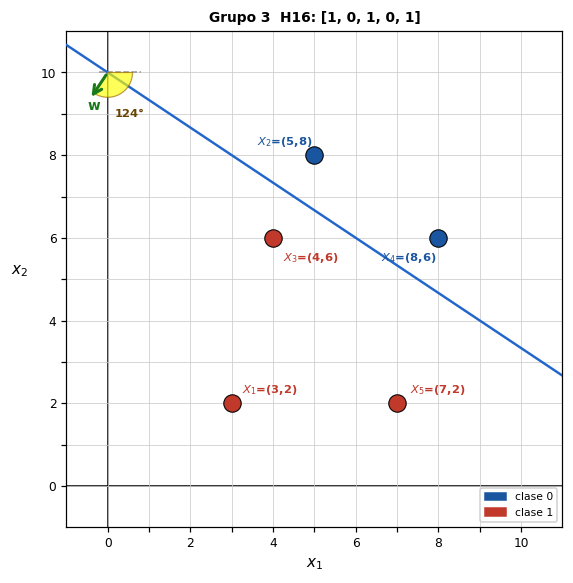
\includegraphics[width=0.65\textwidth]{imagenes_hipotesis/Grupo_3_H16.png}
  \caption{$H_{16}$ -- Grupo 3}
\end{figure}
\textbf{An\'alisis:}
\begin{itemize}
  \item \textbf{Funci\'on separadora:} $-0.50 x_1 - 0.75 x_2 + 7.50 = 0$
  \item \textbf{Vector normal:} $\mathbf{w} = (-0.500, -0.750)$, perpendicular a la recta.
  \item \textbf{\'Angulo:} $\theta = 236.3 grados$.
  \item \textbf{Direcci\'on de $\mathbf{w}$:} El vector $\mathbf{w}$ apunta hacia el \textbf{cuadrante inferior-izquierdo} ($x_1$ negativo, $x_2$ negativo). La clase~1 se encuentra en la regi'on inferior-izquierda.
  \item \textbf{Clase 0} (lado negativo): $X_{2}$, $X_{4}$
  \item \textbf{Clase 1} (lado positivo, direcci\'on de $\mathbf{w}$): $X_{1}$, $X_{3}$, $X_{5}$
\end{itemize}

\subsubsection{Hip\'otesis $H_{17}$: etiquetas [1, 0, 1, 1, 1]}
\begin{table}[H]\centering
  \caption{Clasificaci\'on de $H_{17}$}
  \begin{tabular}{ccc}\toprule
    \textbf{Punto} & \textbf{Coordenadas} & \textbf{Clase}\\\midrule
    $X_{1}$ & (3, 2) & 1 \\
    $X_{2}$ & (5, 8) & 0 \\
    $X_{3}$ & (4, 6) & 1 \\
    $X_{4}$ & (8, 6) & 1 \\
    $X_{5}$ & (7, 2) & 1 \\
  \bottomrule\end{tabular}
\end{table}
\begin{figure}[H]\centering
  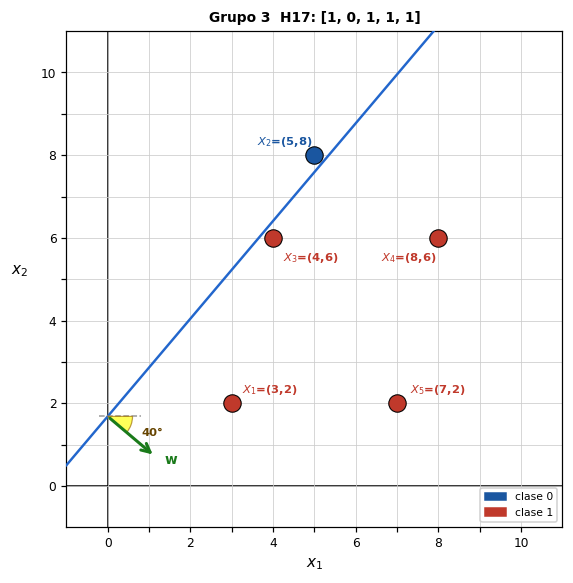
\includegraphics[width=0.65\textwidth]{imagenes_hipotesis/Grupo_3_H17.png}
  \caption{$H_{17}$ -- Grupo 3}
\end{figure}
\textbf{An\'alisis:}
\begin{itemize}
  \item \textbf{Funci\'on separadora:} $2.89 x_1 - 2.44 x_2 + 4.11 = 0$
  \item \textbf{Vector normal:} $\mathbf{w} = (2.889, -2.444)$, perpendicular a la recta.
  \item \textbf{\'Angulo:} $\theta = 319.8 grados$.
  \item \textbf{Direcci\'on de $\mathbf{w}$:} El vector $\mathbf{w}$ apunta hacia el \textbf{cuadrante inferior-derecho} ($x_1$ positivo, $x_2$ negativo). La clase~1 se encuentra en la regi'on inferior-derecha.
  \item \textbf{Clase 0} (lado negativo): $X_{2}$
  \item \textbf{Clase 1} (lado positivo, direcci\'on de $\mathbf{w}$): $X_{1}$, $X_{3}$, $X_{4}$, $X_{5}$
\end{itemize}

\subsubsection{Hip\'otesis $H_{18}$: etiquetas [1, 1, 0, 1, 1]}
\begin{table}[H]\centering
  \caption{Clasificaci\'on de $H_{18}$}
  \begin{tabular}{ccc}\toprule
    \textbf{Punto} & \textbf{Coordenadas} & \textbf{Clase}\\\midrule
    $X_{1}$ & (3, 2) & 1 \\
    $X_{2}$ & (5, 8) & 1 \\
    $X_{3}$ & (4, 6) & 0 \\
    $X_{4}$ & (8, 6) & 1 \\
    $X_{5}$ & (7, 2) & 1 \\
  \bottomrule\end{tabular}
\end{table}
\begin{figure}[H]\centering
  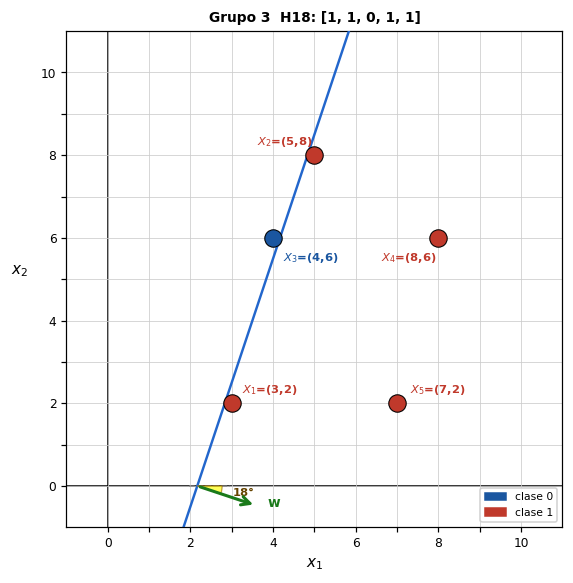
\includegraphics[width=0.65\textwidth]{imagenes_hipotesis/Grupo_3_H18.png}
  \caption{$H_{18}$ -- Grupo 3}
\end{figure}
\textbf{An\'alisis:}
\begin{itemize}
  \item \textbf{Funci\'on separadora:} $6.00 x_1 - 2.00 x_2 - 13.00 = 0$
  \item \textbf{Vector normal:} $\mathbf{w} = (6.000, -2.000)$, perpendicular a la recta.
  \item \textbf{\'Angulo:} $\theta = 341.6 grados$.
  \item \textbf{Direcci\'on de $\mathbf{w}$:} El vector $\mathbf{w}$ apunta hacia el \textbf{cuadrante inferior-derecho} ($x_1$ positivo, $x_2$ negativo). La clase~1 se encuentra en la regi'on inferior-derecha.
  \item \textbf{Clase 0} (lado negativo): $X_{3}$
  \item \textbf{Clase 1} (lado positivo, direcci\'on de $\mathbf{w}$): $X_{1}$, $X_{2}$, $X_{4}$, $X_{5}$
\end{itemize}

\subsubsection{Hip\'otesis $H_{19}$: etiquetas [1, 1, 1, 0, 0]}
\begin{table}[H]\centering
  \caption{Clasificaci\'on de $H_{19}$}
  \begin{tabular}{ccc}\toprule
    \textbf{Punto} & \textbf{Coordenadas} & \textbf{Clase}\\\midrule
    $X_{1}$ & (3, 2) & 1 \\
    $X_{2}$ & (5, 8) & 1 \\
    $X_{3}$ & (4, 6) & 1 \\
    $X_{4}$ & (8, 6) & 0 \\
    $X_{5}$ & (7, 2) & 0 \\
  \bottomrule\end{tabular}
\end{table}
\begin{figure}[H]\centering
  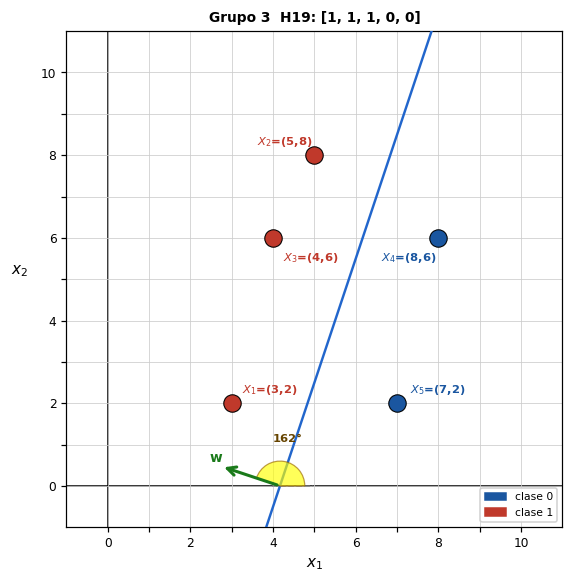
\includegraphics[width=0.65\textwidth]{imagenes_hipotesis/Grupo_3_H19.png}
  \caption{$H_{19}$ -- Grupo 3}
\end{figure}
\textbf{An\'alisis:}
\begin{itemize}
  \item \textbf{Funci\'on separadora:} $-0.55 x_1 + 0.18 x_2 + 2.27 = 0$
  \item \textbf{Vector normal:} $\mathbf{w} = (-0.545, 0.182)$, perpendicular a la recta.
  \item \textbf{\'Angulo:} $\theta = 161.6 grados$.
  \item \textbf{Direcci\'on de $\mathbf{w}$:} El vector $\mathbf{w}$ apunta hacia el \textbf{cuadrante superior-izquierdo} ($x_1$ negativo, $x_2$ positivo). La clase~1 se encuentra a la izquierda y arriba de la frontera.
  \item \textbf{Clase 0} (lado negativo): $X_{4}$, $X_{5}$
  \item \textbf{Clase 1} (lado positivo, direcci\'on de $\mathbf{w}$): $X_{1}$, $X_{2}$, $X_{3}$
\end{itemize}

\subsubsection{Hip\'otesis $H_{20}$: etiquetas [1, 1, 1, 0, 1]}
\begin{table}[H]\centering
  \caption{Clasificaci\'on de $H_{20}$}
  \begin{tabular}{ccc}\toprule
    \textbf{Punto} & \textbf{Coordenadas} & \textbf{Clase}\\\midrule
    $X_{1}$ & (3, 2) & 1 \\
    $X_{2}$ & (5, 8) & 1 \\
    $X_{3}$ & (4, 6) & 1 \\
    $X_{4}$ & (8, 6) & 0 \\
    $X_{5}$ & (7, 2) & 1 \\
  \bottomrule\end{tabular}
\end{table}
\begin{figure}[H]\centering
  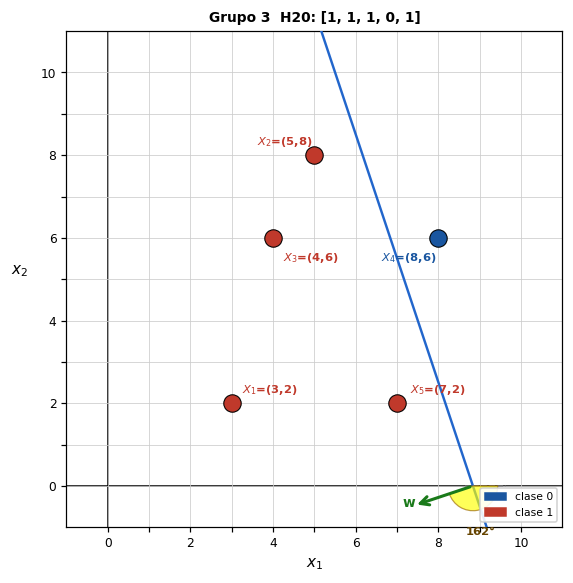
\includegraphics[width=0.65\textwidth]{imagenes_hipotesis/Grupo_3_H20.png}
  \caption{$H_{20}$ -- Grupo 3}
\end{figure}
\textbf{An\'alisis:}
\begin{itemize}
  \item \textbf{Funci\'on separadora:} $-0.86 x_1 - 0.29 x_2 + 7.57 = 0$
  \item \textbf{Vector normal:} $\mathbf{w} = (-0.857, -0.286)$, perpendicular a la recta.
  \item \textbf{\'Angulo:} $\theta = 198.4 grados$.
  \item \textbf{Direcci\'on de $\mathbf{w}$:} El vector $\mathbf{w}$ apunta hacia el \textbf{cuadrante inferior-izquierdo} ($x_1$ negativo, $x_2$ negativo). La clase~1 se encuentra en la regi'on inferior-izquierda.
  \item \textbf{Clase 0} (lado negativo): $X_{4}$
  \item \textbf{Clase 1} (lado positivo, direcci\'on de $\mathbf{w}$): $X_{1}$, $X_{2}$, $X_{3}$, $X_{5}$
\end{itemize}

\subsubsection{Hip\'otesis $H_{21}$: etiquetas [1, 1, 1, 1, 0]}
\begin{table}[H]\centering
  \caption{Clasificaci\'on de $H_{21}$}
  \begin{tabular}{ccc}\toprule
    \textbf{Punto} & \textbf{Coordenadas} & \textbf{Clase}\\\midrule
    $X_{1}$ & (3, 2) & 1 \\
    $X_{2}$ & (5, 8) & 1 \\
    $X_{3}$ & (4, 6) & 1 \\
    $X_{4}$ & (8, 6) & 1 \\
    $X_{5}$ & (7, 2) & 0 \\
  \bottomrule\end{tabular}
\end{table}
\begin{figure}[H]\centering
  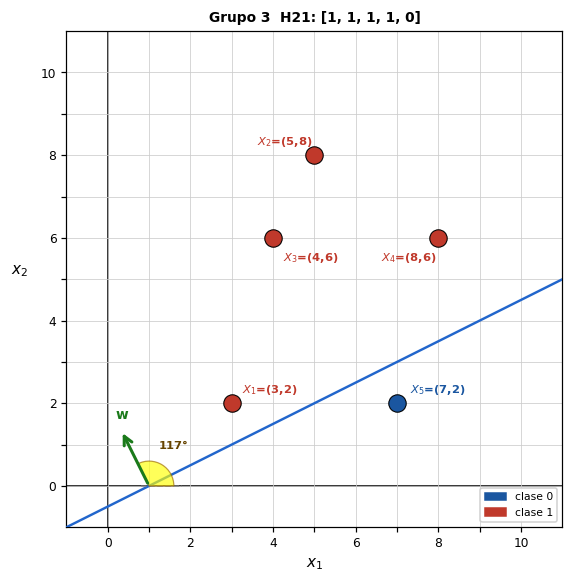
\includegraphics[width=0.65\textwidth]{imagenes_hipotesis/Grupo_3_H21.png}
  \caption{$H_{21}$ -- Grupo 3}
\end{figure}
\textbf{An\'alisis:}
\begin{itemize}
  \item \textbf{Funci\'on separadora:} $-0.50 x_1 + 1.00 x_2 + 0.50 = 0$
  \item \textbf{Vector normal:} $\mathbf{w} = (-0.500, 1.000)$, perpendicular a la recta.
  \item \textbf{\'Angulo:} $\theta = 116.6 grados$.
  \item \textbf{Direcci\'on de $\mathbf{w}$:} El vector $\mathbf{w}$ apunta hacia el \textbf{cuadrante superior-izquierdo} ($x_1$ negativo, $x_2$ positivo). La clase~1 se encuentra a la izquierda y arriba de la frontera.
  \item \textbf{Clase 0} (lado negativo): $X_{5}$
  \item \textbf{Clase 1} (lado positivo, direcci\'on de $\mathbf{w}$): $X_{1}$, $X_{2}$, $X_{3}$, $X_{4}$
\end{itemize}

\subsubsection{Hip\'otesis $H_{22}$: etiquetas [1, 1, 1, 1, 1]}
\begin{table}[H]\centering
  \caption{Clasificaci\'on de $H_{22}$}
  \begin{tabular}{ccc}\toprule
    \textbf{Punto} & \textbf{Coordenadas} & \textbf{Clase}\\\midrule
    $X_{1}$ & (3, 2) & 1 \\
    $X_{2}$ & (5, 8) & 1 \\
    $X_{3}$ & (4, 6) & 1 \\
    $X_{4}$ & (8, 6) & 1 \\
    $X_{5}$ & (7, 2) & 1 \\
  \bottomrule\end{tabular}
\end{table}
\begin{figure}[H]\centering
  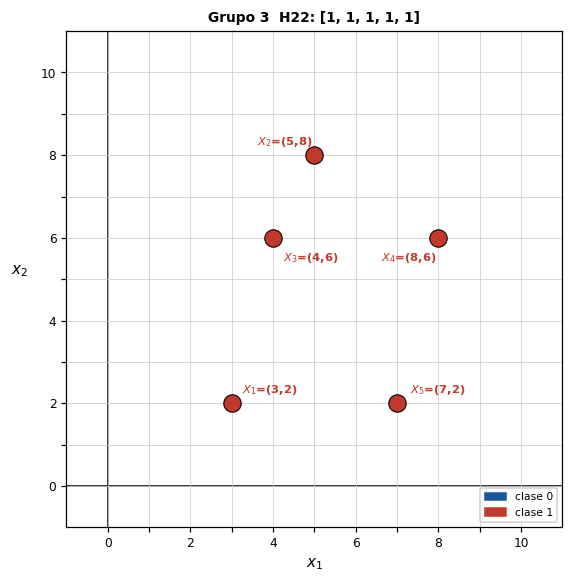
\includegraphics[width=0.65\textwidth]{imagenes_hipotesis/Grupo_3_H22.png}
  \caption{$H_{22}$ -- Grupo 3}
\end{figure}
\textbf{An\'alisis:}
\begin{itemize}
  \item Esta hip\'otesis es \textbf{trivial}: todos los puntos pertenecen a la misma clase.
  \item No existe frontera de decisi\'on expl\'icita.
\end{itemize}

\subsection{Hip\'otesis NO Linealmente Separables}
Las siguientes dic\'otom\'ias \textbf{no pueden ser realizadas}
por ning\'un clasificador lineal sobre este conjunto de puntos.
\begin{figure}[H]\centering
  \begin{subfigure}[b]{0.47\textwidth}
    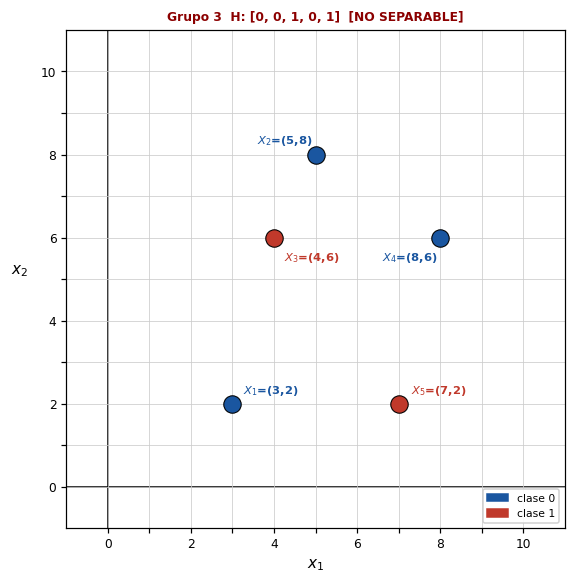
\includegraphics[width=\textwidth]{imagenes_hipotesis/Grupo_3_NS01.png}
    \caption{No separable: [0, 0, 1, 0, 1]}
  \end{subfigure}\hfill
  \begin{subfigure}[b]{0.47\textwidth}
    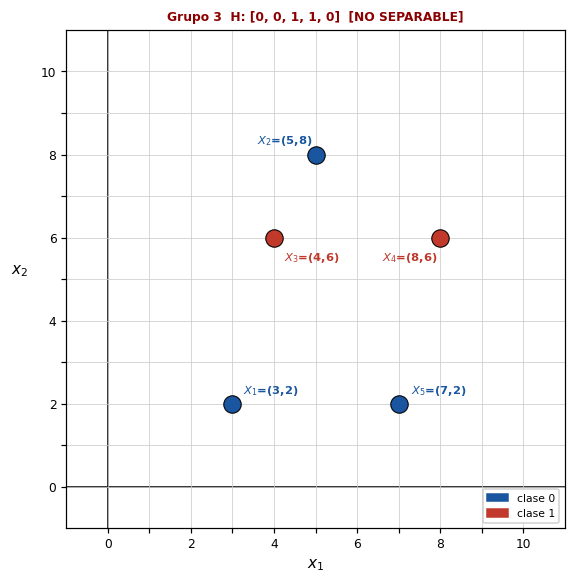
\includegraphics[width=\textwidth]{imagenes_hipotesis/Grupo_3_NS02.png}
    \caption{No separable: [0, 0, 1, 1, 0]}
  \end{subfigure}\hfill
\end{figure}

\begin{figure}[H]\centering
  \begin{subfigure}[b]{0.47\textwidth}
    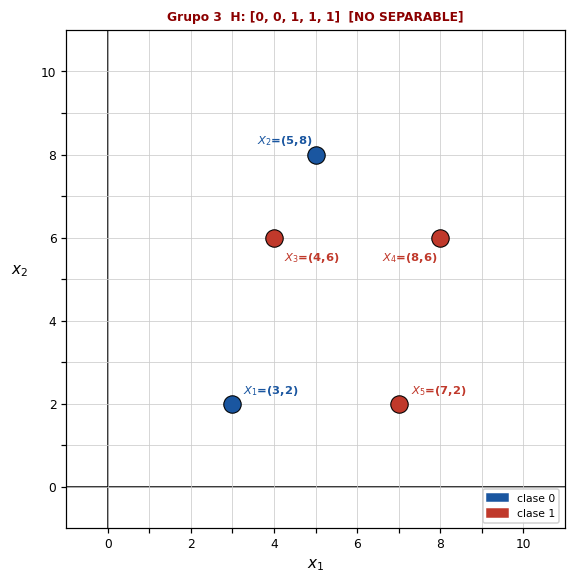
\includegraphics[width=\textwidth]{imagenes_hipotesis/Grupo_3_NS03.png}
    \caption{No separable: [0, 0, 1, 1, 1]}
  \end{subfigure}\hfill
  \begin{subfigure}[b]{0.47\textwidth}
    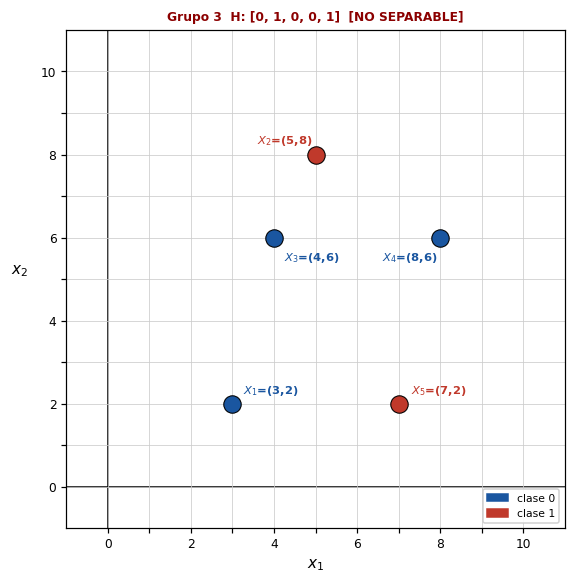
\includegraphics[width=\textwidth]{imagenes_hipotesis/Grupo_3_NS04.png}
    \caption{No separable: [0, 1, 0, 0, 1]}
  \end{subfigure}\hfill
\end{figure}

\begin{figure}[H]\centering
  \begin{subfigure}[b]{0.47\textwidth}
    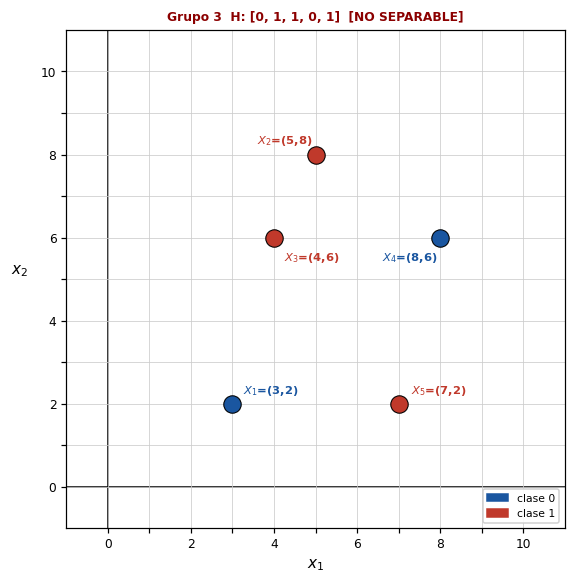
\includegraphics[width=\textwidth]{imagenes_hipotesis/Grupo_3_NS05.png}
    \caption{No separable: [0, 1, 1, 0, 1]}
  \end{subfigure}\hfill
  \begin{subfigure}[b]{0.47\textwidth}
    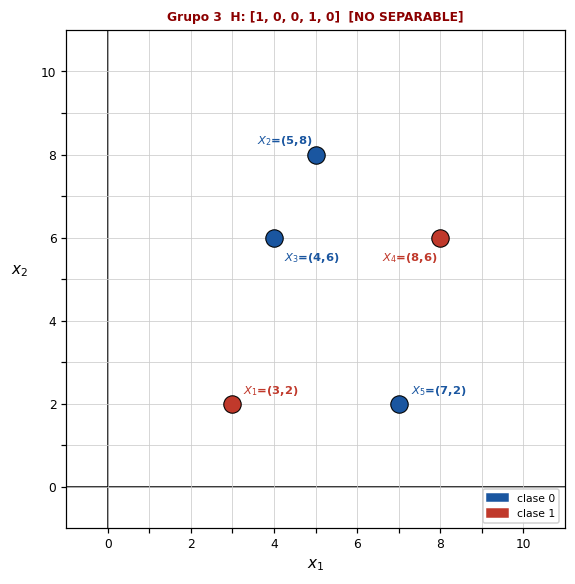
\includegraphics[width=\textwidth]{imagenes_hipotesis/Grupo_3_NS06.png}
    \caption{No separable: [1, 0, 0, 1, 0]}
  \end{subfigure}\hfill
\end{figure}

\begin{figure}[H]\centering
  \begin{subfigure}[b]{0.47\textwidth}
    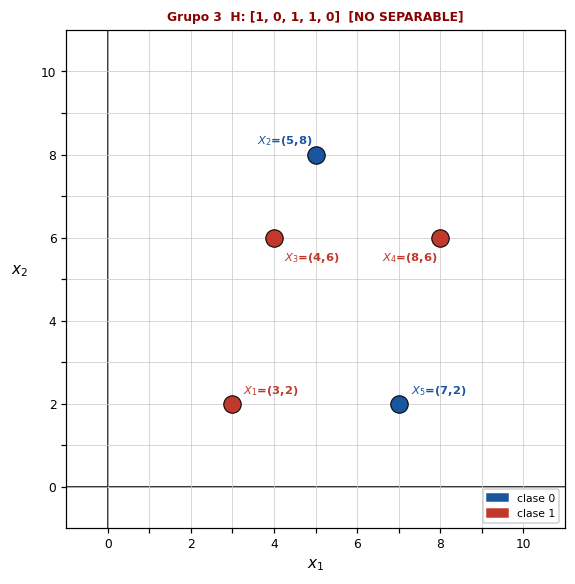
\includegraphics[width=\textwidth]{imagenes_hipotesis/Grupo_3_NS07.png}
    \caption{No separable: [1, 0, 1, 1, 0]}
  \end{subfigure}\hfill
  \begin{subfigure}[b]{0.47\textwidth}
    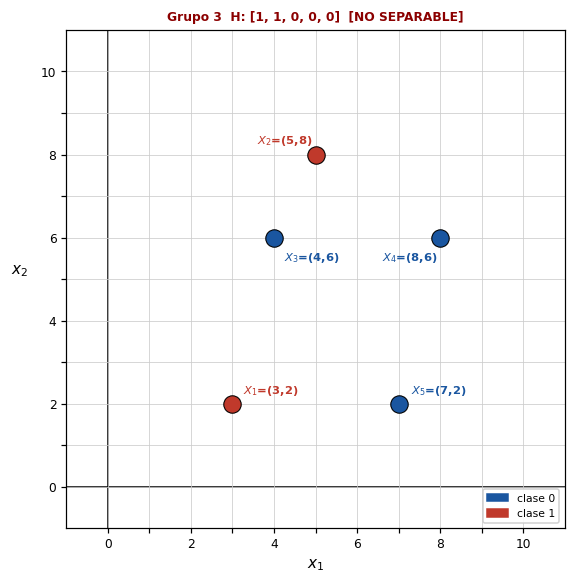
\includegraphics[width=\textwidth]{imagenes_hipotesis/Grupo_3_NS08.png}
    \caption{No separable: [1, 1, 0, 0, 0]}
  \end{subfigure}\hfill
\end{figure}

\begin{figure}[H]\centering
  \begin{subfigure}[b]{0.47\textwidth}
    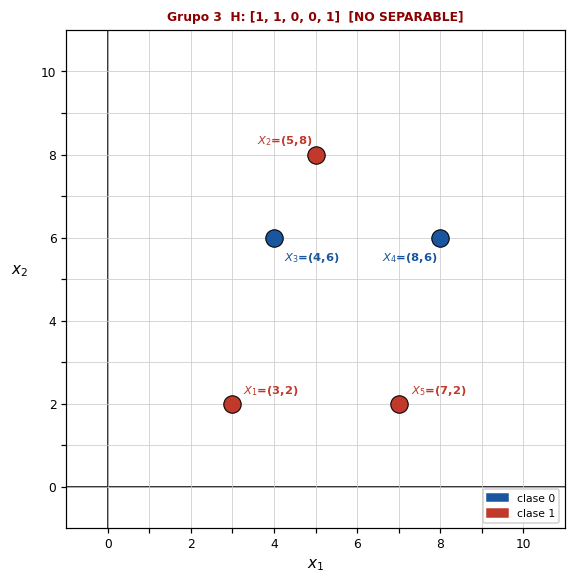
\includegraphics[width=\textwidth]{imagenes_hipotesis/Grupo_3_NS09.png}
    \caption{No separable: [1, 1, 0, 0, 1]}
  \end{subfigure}\hfill
  \begin{subfigure}[b]{0.47\textwidth}
    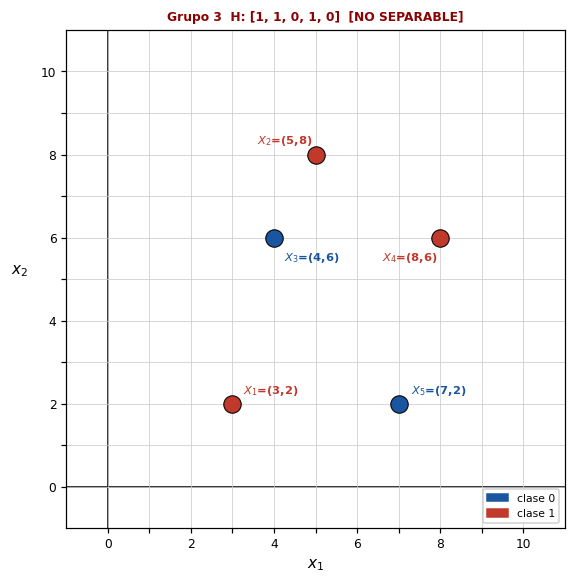
\includegraphics[width=\textwidth]{imagenes_hipotesis/Grupo_3_NS10.png}
    \caption{No separable: [1, 1, 0, 1, 0]}
  \end{subfigure}\hfill
\end{figure}


\section{An\'alisis Comparativo}
\begin{table}[H]\centering
  \caption{Funci\'on de crecimiento $m_{\mathcal{H}}(N)$}
  \begin{tabular}{lccc}\toprule
    \textbf{Grupo} & \textbf{N} & \textbf{$2^N$} & \textbf{Separables}\\\midrule
    Grupo 1 & 4 & 16 & 12 \\
    Grupo 2 & 4 & 16 & 14 \\
    Grupo 3 & 5 & 32 & 22 \textbf{(max)} \\
  \bottomrule\end{tabular}
\end{table}

\begin{enumerate}
  \item \textbf{Grupo 2:} presenta el patr\'on XOR. La dic\'otom\'ia $[0,1,1,0]$
        y $[1,0,0,1]$ \textbf{no son linealmente separables}, lo que ilustra
        la limitaci\'on fundamental de los clasificadores lineales.
  \item \textbf{Grupo 1:} puntos casi colineales en $x_2 \approx x_1$,
        lo que permite varias rectas separadoras con distinta pendiente.
  \item \textbf{Grupo 3:} con $N=5$ tiene el mayor espacio de dic\'otom\'ias posibles.
\end{enumerate}

\section{Conclusiones}
\begin{enumerate}
  \item El vector $\mathbf{w}$ es siempre perpendicular a la frontera de decisi\'on
        y apunta hacia la regi\'on de clase~1.
  \item El \'angulo $\theta$ indica la orientaci\'on positiva de la hip\'otesis.
  \item Configuraciones como el XOR no son linealmente separables y
        requieren modelos no lineales (kernels, redes neuronales).
  \item La funci\'on de crecimiento $m_{\mathcal{H}}(N)$ mide la capacidad
        del clasificador lineal sobre un conjunto dado de puntos.
\end{enumerate}
\end{document}
